\documentclass[BCOR=12mm,DIV11,titlepage,a4paper,oneside]{scrbook}

%Paket für deutsche Silbentrennung etc.
\usepackage{ngerman}

%Paket für Zeichenkodierung, entspricht UTF-8
\usepackage[utf8x]{inputenc}

%Paket das die Ausgabefonts definiert
\usepackage[T1]{fontenc}

%Paket für Sonderzeichen wir RightsReserved
\usepackage{textcomp}

%Euro-Symbol
\usepackage[right]{eurosym}

% Matheumgebung
\usepackage[]{framed, amsmath}

%Paket für das Einbinden von Grafiken über die figure-Umgebung
\usepackage{graphicx}

%Paket zum Ändern der Kopf- und Fußzeile
\usepackage{fancyhdr}
%Benutzt das Paket für eigenen Seitenstil
\pagestyle{fancy} 
%Erzeugt eine Linie in der Kopfzeile (lässt sich mit 0.0pt ausblenden)
\renewcommand*{\headrulewidth}{0.8pt} 
\renewcommand*{\headrule}{\hbox to\headwidth{%
    \color{thmagenta}\leaders\hrule height \headrulewidth\hfill}}
\fancyhf{}
\fancyhead[EC,OC]{\thepage}
% \fancyhead[EL]{\leftmark} 
% \fancyhead[OR]{\rightmark} 
% \fancyhead[ER,OL]{\thepage}
\renewcommand{\sectionmark}[1]{ 
\markboth{\thechapter{} #1}{\thechapter{} #1} 
}
% Ermöglicht ToDos ansprechend zu setzen
\usepackage{xargs} 
\usepackage[colorinlistoftodos,prependcaption,textsize=tiny]{todonotes}
\newcommandx{\unsure}[2][1=]{\todo[linecolor=red,backgroundcolor=red!25,bordercolor=red,#1]{#2}}
\newcommandx{\change}[2][1=]{\todo[linecolor=blue,backgroundcolor=blue!25,bordercolor=blue,#1]{#2}}
\newcommandx{\info}[2][1=]{\todo[linecolor=OliveGreen,backgroundcolor=OliveGreen!25,bordercolor=OliveGreen,#1]{#2}}
\newcommandx{\improvement}[2][1=]{\todo[linecolor=Plum,backgroundcolor=Plum!25,bordercolor=Plum,#1]{#2}}
\newcommandx{\thiswillnotshow}[2][1=]{\todo[disable,#1]{#2}}

%Ändert die Seitennummerierung beim Inhaltsverzeichnis mit eigenem Stil
\renewcommand*{\indexpagestyle}{fancy}
%Verhindert die Seitennummerierung auf den Part-Seiten
\renewcommand*{\partpagestyle}{empty}
%Ändert die Seitennummerierung bei Chapter mit eigenem Stil
\renewcommand*{\chapterpagestyle}{fancy}

%Abbildungsnummerierung ändern (abhängig von chapter, z.B. Abbildung 1.1)
\renewcommand*{\thefigure}{\thechapter.\arabic{figure}}
%Tabellennummerierung ändern (abhängig von chapter, z.B. Tabelle 1.1)
\renewcommand*{\thetable}{\thechapter.\arabic{table}}

%Paket, um ein Glossar/Abkürzungsverzeichnis anzulegen
\usepackage[intoc]{nomencl}
\let\abbrev\nomenclature
%Der Name wird in Glossar geändert
\renewcommand{\nomname}{Glossar}
%Definiert die Aufteilung im Glossar zwischen Begriffen und Erläuterung
\setlength{\nomlabelwidth}{.25\hsize}
%Definiert die Punktelinien im Glossar
\renewcommand{\nomlabel}[1]{#1 \dotfill}
\setlength{\nomitemsep}{-\parsep}
%Veranlasst die Erstellung des Glossars
\makenomenclature

%Einrückungen nach Absätzen und Grafiken verhindern
\setlength{\parindent}{0pt}

\usepackage[nohyperlinks, printonlyused, withpage, smaller]{acronym}


%Verhindern, dass eine neue Seite für ein einzelnes Wort/Zeile verwendet wird
\clubpenalty = 10000 % schliesst Schusterjungen aus 
\widowpenalty = 10000 % schliesst Hurenkinder aus (keine Beleidigung, sondern wirklich ein Fachbegriff)

%Paket für ein deutsches Literaturverzeichnis
\usepackage[authoryear,round]{natbib}
\bibliographystyle{natdin}
% \setlength\bibhang{30pt}

%Paket für die Verwendung von URLs durch den Befehl \url{}
\usepackage{url}

%Paket für Zeilenabstand (onehalfspace, singlespace)
\usepackage{setspace}

%Paket zur Erzeugung von Anführungszeichen durch \enquote{Text}
\usepackage[ngerman]{babel}
\usepackage[babel, german=quotes]{csquotes}

%Paket für farbigen Text
%black,white,green,red,blue,yellow,cyan,magenta
\usepackage{color}
%Farbige Tabellen
\usepackage{colortbl}

%Rotation von Gleitobjekten (Grafiken, Trabellen, etc.)
\usepackage{rotating}

%Rotation von einzelnen Seiten begin{landscape}
\usepackage{lscape}

%Paket für farbigen Hintergrund für Verbatim-Umgebung (Quelltext-Umgebung)
\usepackage{fancyvrb}
\usepackage{verbatim,moreverb}
%Grauton für Quelltext-Umgebung definieren 80% Grau
\definecolor{sourcegray}{gray}{.80}

%Definition der TH Köln-Farben
\definecolor{thred}{cmyk}{0.0,1.0,1.0,0.15}
\definecolor{thorange}{cmyk}{0.0,0.75,1.0,0.0}
\definecolor{thmagenta}{cmyk}{0.3,0.95,0.0,0.0}
\definecolor{thblack}{cmyk}{0.0,0.0,0.0,1.0}

%Paket für Quelltext-Umgebung
\usepackage{listings}
%Alternative Quelltext-Umgebung
%\lstset{numbers=left, 
%	numberstyle=\tiny, 
%	numbersep=5pt,
%	language=Java,
%	breaklines=true,
%	breakautoindent=true,
%	postbreak=\space,
%	tabsize=2,
%	frame=tlrb,
%	basicstyle=\ttfamily\footnotesize}

\usepackage{tikz}

\tikzstyle{sourcecodebox} = [
    draw=blue, very thick,
    rectangle, rounded corners,
    inner sep=10pt
]
\tikzstyle{sourcecodetitle} = [
    fill=black, text=white,
    rectangle, rounded corners
]

\makeatletter
\lstnewenvironment{javacode}[1][]{%
    \def\javacodetitle{#1}%
    \lstset{%
        language=java,
        basicstyle=\ttfamily\footnotesize,
        escapeinside={(*@}{@*)},
        %numbers=left,
        breaklines=true,
        breakatwhitespace=true,
        showspaces=false,
        showstringspaces=false,
        frame=shadowbox,
        frameround=rrrt,
        keywordstyle=\color{blue}\ttfamily,
        commentstyle=\color{comment}\ttfamily,
        linewidth=.95\textwidth,
        rulecolor=\color{black},
        rulesepcolor=\color{gray}
    }%
    \setbox\@tempboxa=\hbox\bgroup\color@setgroup
}%
{%
    \color@endgroup\egroup
    \begin{tikzpicture}
        \node[sourcecodebox] (box)
            % Makebox is needed to take the frame added by listings into account
            {\makebox[.95\textwidth][l]{\box\@tempboxa}};
        \node[sourcecodetitle] at (box.north) 
        {\javacodetitle};
    \end{tikzpicture}
}

% Implementierung innerhalb des Dokumentes
%\begin{javacode}[Initialisierung AlchemyAPI]
%public static AlchemyAPI alchemyObj;
%
%public static void init() {
%    alchemyObj = AlchemyAPI.GetInstanceFromString(KEY);
%}
%
%\end{javacode}

%Paket für Positionierung der Objekte ohne Float (Verwendungsbsp.: \begin{figure}[H])
%\usepackage{here}
%Alternatives Paket für here.sty
\usepackage{float}

%DRAFT als Wasserzeichen im Hintergrund
% \usepackage{draftwatermark} 
% \SetWatermarkAngle{60}
% \SetWatermarkScale{5.0}

%Für lange Tabellen
\usepackage{longtable,array,supertabular}

%Für rowspan in Tabellen
\usepackage{multirow}

%Behält die Schriftgröße der Überschrift normal, wenn z.B. die Schriftgröße in einer Tabelle verändert wird
\addtokomafont{caption}{\normalsize} 

%Paket um PDF Seiten einzubinden
\usepackage{pdfpages}

%Paket zur Erzeugung von Hyperrefs und PDF Informationen
\usepackage[pdftex,plainpages=false,pdfpagelabels,
            pdftitle={title},
            pdfauthor={name}
            ]{hyperref}
%Farben für Links
%Farbige Ränder bei false und farbige Texte bei true
\hypersetup{colorlinks=true,citecolor=black,filecolor=black,linkcolor=black,urlcolor=black}

\apptocmd{\UrlBreaks}{\do\f\do\m}{}{}

%Zwei Verzeichnisse für Inhalt und Anhang
\usepackage{appendix}
% \usepackage{minitoc} 
% \nomtcrule
% \renewcommand{\mtctitle}{Anhangsverzeichnis}
% \setlength{\mtcindent}{0pt} 

\begin{document}

%=== Einleitung ======================================================
\frontmatter 
\setcounter{page}{3}
\pagenumbering{arabic}

%!TEX root = ../draft.tex
\begin{titlepage}
\newcommand{\distance}{1.2cm}
\begin{center}
%Logo der Fachhochschule Köln
\begin{figure*}[!ht]
	\flushright
		
\includegraphics[width=.2\textwidth]{images/logo.pdf}
		
\includegraphics[width=\textwidth]{images/balken.png}
\end{figure*}

\vspace{\distance}

%Deutscher Titel
\begin{rmfamily}
\begin{huge}
\textbf{Anforderungsanalyse }\\	
\end{huge}
\vspace{0.5cm}
\begin{LARGE}
für ein\\ Praktikums-Management-Werkzeug zum Einsatz in heterogenen Laborstrukturen\\
\end{LARGE}
\end{rmfamily}

\vspace{1.0cm}

%Englischer Titel
% \begin{rmfamily}
% \textbf{\LARGE Title in English}\\
% \large with a very\\long subtitle\\
% \normalsize
% \end{rmfamily}

% \vspace{1.2cm}

%Bachelorarbeit 
\begin{LARGE}
\begin{scshape}
Praxisprojekt\\[0.6em]
\end{scshape}
\end{LARGE}

%ausgearbeitet von...
\begin{large}
ausgearbeitet von\\
\begin{LARGE}
Florian Herborn\\
\end{LARGE}
\end{large}

\vspace{1.0cm}

%zur Erlangung des akademischen Grades...
%\begin{large}
%zur Erlangung des akademischen Grades\\
%\vspace{0.2cm}
%\textsc{Master of Science (B.Sc.)}\\ 
%\end{large}

%\vspace{0.4cm}

%vorgelegt an der...
\begin{large}
vorgelegt an der\\ 
\vspace{0.2cm}
\begin{scshape}
Technische Hochschule Köln\\
Campus Gummersbach\\
Fakultät für Informatik und\\
Ingenieurwissenschaften\\
\end{scshape}
\end{large}

\vspace{0.4cm}

%im Studiengang...
\begin{large}
im Studiengang\\ 
\vspace{0.2cm}
\textsc{Allgemeine Informatik}
\end{large}


\vspace{1.0cm}

%Autor der Bachelorarbeit und die Prüfer
\begin{tabular}{rl}
        Prüfer:  &  Prof. Dr. Christian Kohls\\
       					&  \small Technische Hochschule Köln \\[1.0em]
\end{tabular}

\vspace{0.8cm}

%Ort, Monat der Abgabe
\begin{large}
Gummersbach, im Juni 2017
\end{large}
\vspace{\distance}
\end{center}
\begin{figure*}[!ht]
		
\includegraphics[width=\textwidth]{images/balken.png}
\end{figure*}

%!TEX root = ../draft.tex
\thispagestyle{empty}

%Kontaktmöglichkeiten des Autors und der Prüfer
\begin{center}
\begin{tabular}{rl}
							&  \\[30.0em]
							&  \quad 
\includegraphics[width=.2\textwidth]{images/logo}\\
							&  \\[2.0em]
							
\large \textbf{Adressen:}	&  	\quad Florian Herborn\\
							&  	\quad Parkweg 8\\
							&	\quad 51491 Overath\\
							&  	\quad florianHerborn2293@t-online.de\\[2.0em]
							
							&  	\quad Prof. Dr. Christian Kohls\\
							&  	\quad Technische Hochschule Köln\\
							&  	\quad Institut für Informatik\\
							&	\quad Steinmüllerallee 1\\
							&	\quad 51643 Gummersbach\\
							&  	\quad christian.kohls@th-koeln.de\\[2.0em]
\end{tabular}
\end{center}

\end{titlepage}


\onehalfspacing
%!TEX root = ../draft.tex
\chapter*{Kurzfassung}

Das Ziel der vorliegenden Arbeit war es, Anforderungen für das \ac{LWM} des ADV-Labors zu ermitteln. Dazu wurden 13 ausgewählte, potentielle Stakeholder in Interviews über ihre Wünsche und Interessen, die dieses Tool betreffen, befragt. Die so gesammelten Erkenntnisse wurden anschließend ausgewertet, um als Grundstein für die weitere Entwicklung des Tools zu dienen. Dazu wurden diese mittels User-Storys dokumentiert und mit Story-Points und Kano-Faktoren bewertet und priorisiert. Des Weiteren wurde eine Webseite entwickelt, die zahlreiche Funktionalitäten zur Verarbeitung der Anforderungen bereitstellt. Die Ergebnisse dieser Arbeit zeigen, dass in dem aktuellen LWM noch viel Potential steckt, welches, mit der Umsetzung einiger dieser Anforderungen, gefördert werden kann. Diese Arbeit ist deshalb, sowohl für Studierende der Informatik, als auch für Lehrende in diesem Bereich und Nutzer des LWM, interessant.


\singlespacing
%!TEX root = ../draft.tex

%Für Anhangsverzeichnis
% \dominitoc

\tableofcontents
\onehalfspacing

%=== Hauptteil =======================================================
\mainmatter
\setcounter{page}{6}

%Einbinden eines Vorwortes
%!TEX root = ../draft.tex
\chapter*{Vorwort}
\addcontentsline{toc}{chapter}{Vorwort}

Vor Ihnen liegt das Praxisprojekt \glqq Anforderungsanalyse für ein Praktikums-Management-Werkzeug zum Einsatz in heterogenen Laborstrukturen\grqq . Die in dieser Dokumentation beschriebene Forschungsarbeit wurde in enger Zusammenarbeit mit dem Entwickler-Team des LWM durchgeführt, in dem auch ich seit einem Jahr als Backend-Entwickler tätig bin.\\

Für das entgegengebrachte Engagement möchte ich meinen Kollegen Uwe Müsse und
Alexander Dobrynin danken. Ohne ihr Zutun wäre ein großer Teil des hier erreichten Ergebnisses nicht in dieser Form zustande gekommen. Auch haben sie mir in schwierigen Situationen Hilfestellungen und Denkansätze gegeben.\\

Im Laufe des Projekts wurden zahlreiche Interviews mit Modulverantwortlichen und ihren Mitarbeitern geführt. Diese Gespräche haben im Schnitt 1 - 1,5 Stunden gedauert, trotzdem haben mir die Beteiligten bereitwillig zur Verfügung gestanden, weshalb auch ihnen mein Dank gilt. Ohne sie wäre der Kern dieser Arbeit nicht realisierbar gewesen.\\

Ein weiterer Dank gebührt meiner Freundin, die mir während den Abschlussarbeiten den Rücken frei gehalten hat. Nur so war es mir Möglich, diese rechtzeitig fertigzustellen.\\

Ich wünsche Ihnen viel Spaß beim Lesen.\\

Florian Herborn

	% Die Zähler für Tabellen und Abbildungen werden zurückgesetzt, damit
	% in jedem Kapitel die Nummerierung neu beginnt
\setcounter{table}{1}
\setcounter{figure}{1}
	% \include{chapter/mathetest} 
	%!TEX root = ../draft.tex
\chapter{Motivation}

\section{Ausgangssituation}

Das aktuelle \ac{LWM} wurde für die Praktika des ADV-Labors am Campus Gummersbach der TH-Köln entwickelt. Ziel des Tools ist es, die Massenabfertigung eines Praktikums zu vereinfachen. Dies soll erreicht werden, indem der Staffelplan des Praktikums automatisch generiert wird und im Zuge dessen Konflikte mit anderen Praktika bestmöglich eliminiert werden. Es bietet zudem die Möglichkeit, Praktikumsteilnehmern die Anwesenheit an einem Termin, seine Leistungen sowie die erlangten Bonuspunkte zu vermerken.

\section{Problemstellung}

Da das \ac{LWM} in erster Linie für das ADV-Labor entwickelt wurde, deren Praktika eine gleichbleibende Struktur aufwiesen, wurde das Tool genau für dieses Praktikumsschema modelliert. Mittlerweile hat sich die Struktur der Praktika des ADV-Labors verändert und es nutzen zunehmend mehr Außenstehende Module das LWM. Deshalb ist das Tool zum derzeitigen Stand nicht mehr in der Lage, die Anforderungen der Nutzer optimal zu erfüllen.

\section{Lösungsansatz}

Um herauszufinden welche Funktionalitäten das \ac{LWM} beinhalten muss, damit es den Anforderungen aller Nutzer entspricht, ist ein Verfahren notwendig, welches die Wünsche und Meinungen der Nutzer in die Planung miteinbezieht. Dafür bietet sich eine Anforderungsanalyse an, diese Ergebnisse können dann zur Verbesserung der Nutzbarkeit des Tools beitragen. Mit einer anschließenden Aufwandsschätzung und Priorisierung können die wichtigsten Anforderungen herausgefiltert werden, um sie daraufhin umzusetzen.




\nomenclature{Staffelplan}{Ein Terminplan für das Praktikum in dem alle Termine mit den dazugehörigen Gruppen / Praktikumsteilnehmer eingetragen sind.\vspace{4mm}}

\nomenclature{Modul}{Ein Modul aus dem Modulhandbuch der TH-Köln.\vspace{4mm}}

\nomenclature{Bonuspunkte}{Eine Prüfungsleistung in Punkten, die der Praktikumsteilnehmer während des Praktikums durch seine Leistungen sammeln kann. \vspace{4mm}}































%======================================================================
%======================================================================
% Eintrag ins Glossar
\nomenclature{Stakeholder}{
Ein Stakeholder ist eine Person, Organisation oder Gruppe von Personen, die am Projekt aktiv beteiligt ist oder durch den Projektverlauf oder das Projektergebnis beeinflusst wird (sowohl positiv wie auch negativ), oder die den Projektverlauf oder das Projektergebnis beeinflussen kann (auch dies positiv oder negativ). \citep{GLOSS}
\vspace{4mm}
\label{gloss:stakeholder}
}

\nomenclature{Anforderung}{
Eine Anforderung (engl. Requirement) ist eine Aussage über eine zu erfüllende Eigenschaft (einem Ziel) oder zu erbringende Leistung eines Produktes, Systems oder Prozesses. Also etwas, das das Zielprodukt/-system können muss. \citep{GLOSS}
\vspace{4mm}
\label{gloss:anforderung}
}

\nomenclature{Ziel}{
Ein Ziel bezeichnet einen in der Zukunft liegenden, gegenüber dem Heutigen im allgemeinen veränderten, angestrebten Zustand. Ein Ziel ist somit ein definierter und angestrebeter Endpunkt eines Prozesses. \citep{GLOSS}
\vspace{4mm}
\label{gloss:ziel}
}

\nomenclature{Funktionale Anforderungen}{
Funktionale Anforderungen beschreiben gewünschte Funktionalitäten (was soll das System tun/können) eines Systems bzw. Produkts, dessen Daten oder Verhalten \citep{GLOSS}
\vspace{4mm}
\label{gloss:funktionaleanforderungen}
}

\nomenclature{Qualitätseigenschaften}{
Qualitätseigenschaften beschreiben die "Qualität" in welcher die geforderte Funktionalität zu erbringen ist.
\vspace{4mm}
\label{gloss:qualitätseigenschaft}
}

\nomenclature{Randbedingung}{
Eine Randbedingung ist eine Bedingung die Einfluss auf das Projekt haben kann.
\vspace{4mm}
\label{gloss:randbedingung}
} 

	% Die Zähler für Tabellen und Abbildungen werden zurückgesetzt, damit
	% in jedem Kapitel die Nummerierung neu beginnt
\setcounter{table}{1}
\setcounter{figure}{1}
	% Einbinden des zweiten Kapitels
	%!TEX root = ../draft.tex
\chapter{Theorie}

\section{\acl{RE}}
Im \ac{RE} werden die Anforderungen an ein Produkt, einen Prozess oder am Prozess beteiligte Personen definiert. Die daraus resultierenden Erkenntnisse dienen als Leitfaden für das zu entwickelnde System. \\
Mit dem \ac{RE} wird dafür gesorgt, dass das Endprodukt des Projektes auch den geforderten Anforderungen entspricht. Ist das nicht der Fall, führt dies in der Regel dazu, dass ein Projekt nicht den gewünschten Erfolg bringt. Gerade deshalb ist dem \ac{RE} ein angemessenes Maß an Aufmerksamkeit zu widmen.

\subsection{Einfluss von \acl{RE} auf das Projekt}
Bei dem \ac{RE} werden die Wünsche der Stakeholder schon in der Planungsphase in das Projekt mit einbezogen und berücksichtigt. So können die Funktionalitäten genau auf die Nutzer des Systems abgestimmt und klar definiert werden. Diese Tatsache macht das \ac{RE} zu einem wichtigen Abschnitt in der Entwicklung eines Software-Projektes. Auch in existierenden Systemen kann das \ac{RE} für eine Verbesserung der Usability und Stakeholder-Zufriedenheit sorgen, weshalb es in vielen Projekten in mehreren Iterationen ausgeführt wird. Die Anforderungen können nach der Umsetzung mit Techniken der \ac{MCI} getestet werden, um herauszufinden, ob sie auch tatsächlich der Intention der Nutzer entsprechen und für diese nutzbar umgesetzt wurden.

\section{Stakeholder}
Als Stakeholder werden, wie \cite{FLEIG1} definiert, alle Personen, Gruppen oder Institutionen bezeichnet, die von den Aktivitäten eines Unternehmens direkt oder indirekt betroffen sind oder die irgendein Interesse an diesen Aktivitäten haben.\\

Es gibt drei Arten von Stakeholdern \citep{Schaefer2}, primäre-, sekundäre- und tertiäre Stakeholder.
Die Unterscheidung liegt hier vor allem bei der Größe des Bezugs zum Projekt. 

\subsubsection{Primäre Stakeholder}
Die primären Stakeholder werden, wie auch \cite{FANTA1} berichtet, manchmal als \textit{"die wichtigsten Beteiligten"} bezeichnet. Diese Gruppe besteht aus den Beteiligten, welche den engsten Bezug zu dem Zielsystem haben. Aus diesem Grund haben deren Anforderungen auch den größten Einfluss. Wenn diese Anforderungen nicht erfüllt werden, verliert das Ziel-System die wichtigste Nutzer-Gruppe.

\subsubsection{Sekundäre Stakeholder}
Im Gegensatz zu den primären stehen sekundäre Stakeholder nur indirekt in einer Beziehung zu dem Projekt. Nehmen wir an, es würde ein Mehrfamilienhaus gebaut werden, so wären sowohl die zukünftigen Bewohner dieses Hauses als auch der Bauherr primäre Stakeholder, lokale Baufirmen, welche gegebenenfalls durch dieses Projekt einen Auftrag bekommen könnten, die sekundären.

\subsubsection{Tertiäre Stakeholder}
Tertiäre Stakeholder, auch \textit{"externe"} genannt, stehen auf dem ersten Blick in keinem Bezug zu dem Projekt. Jedoch kann es sein, dass es Personen, Gruppen oder Organisationen gibt, welche dennoch ein berechtigtes Interesse an einem solchen Projekt haben. Dies könnten neben Behörden auch öffentliche Personen oder Organisationen sein. In dem zuvor genannten Beispiel des Bau eines Mehrfamilienhauses, stellt das Bauamt einen tertiären Stakeholder dar. Gehen wir weiter davon aus, dass das Mehrfamilienhaus besonders umweltschonend gebaut werden soll, so könnten auch Umweltaktivisten als Stakeholder in Betracht gezogen werden, da diese zwar nicht direkt mit dem Bau dieses Hauses oder dem Ergebnis in Verbindung stehen, sie dennoch ein berechtigtes Interesse an der Angelegenheit haben.

\section{Anforderungen}
Anforderungen sind Wünsche und Voraussetzungen an die Funktionalität, Qualität und Randbedingungen, die Stakeholder von einer Anwendung fordern.
Diese Anforderungen haben Einfluss auf die Usability und den Erfolg eines Projektes. Werden beispielsweise wichtige Anforderungen nicht erfüllt, führt dies dazu, dass die Nutzer unzufrieden sind oder sogar auf alternative Anwendungen zurückgreifen. Anforderungen sind nicht nur Funktionen, die die Stakeholder sich wünschen, sondern auch Qualitätsmerkmale die vorausgesetzt werden. Auch Gesetze oder andere Randbedingungen können zu Anforderungen werden, sofern sie einen Einfluss auf das Projekt oder dessen Ergebnis haben. Grob wird unterschieden zwischen funktionalen Anforderungen und nicht-funktionalen Anforderungen, welche in den nächsten Abschnitten näher erklärt werden.

\subsection{Funktionale Anforderungen}
\label{subsec:funktionaleanforderungen}
Unter funktionalen Anforderungen versteht man im Software-\ac{RE} Funktionen, welche von dem Zielsystem ausgeführt oder bereitgestellt werden sollen. Jedoch werden auch Systeminteraktionen, die dem Nutzer zur Verfügung stehen, darunter zusammengefasst.\\

Beispiele für funktionale Anforderungen sind:

\begin{quote}
\textit{"Das System soll Usern eine Anmeldung über Facebook ermöglichen."}
\end{quote}
oder 
\begin{quote}
\textit{"Das System muss es dem Administrator ermöglichen, bei der Erstellung eines Kurses die Raumnummer, in dem dieser Kurs stattfinden soll, einzugeben."}
\end{quote}
oder ein weiteres Beispiel
\begin{quote}
\textit{"Der User ist für den Kommunikationsaufbau zum Support zuständig."}
\end{quote}

\subsection{Nicht-Funktionale Anforderungen}
Nicht-funktionale Anforderungen beschreiben, in welcher Art und Qualität das System die geforderte Leistung erbringen soll. Dazu ist es notwendig in zwei weiteren Subkategorien zu unterscheiden: Qualitätseigenschaften und Randbedingungen. 

\subsubsection{Qualitätseigenschaften}
\label{subsubsec:qualitätseigenschaften}
Mit einer Qualitätseigenschaft wird die "Qualität", in welcher die Anforderung erbracht werden soll, beschrieben. Diese Anforderungen können sich sowohl auf die Performanz als auch auf  Zuverlässigkeit, Wartbarkeit oder Portabilität beziehen.\\

Auch hier sind weitere Kategorien zu unterscheiden: technische Anforderungen, welche das System direkt beschreiben und ergonomische Anforderungen, welche eher die Ergebnisse und Darstellungen des Systems beschreiben. 

Ein Beispiel für eine technische Anforderung ist:
\begin{quote}
\textit{"Das Zielsystem muss mit Java entwickelt werden."}
\end{quote}
Eine ergonomische Anforderung hingegen könnte wie folgt lauten:
\begin{quote}
\textit{"Das System muss die Statistik in einem angemessenen Format ausgeben"}
\end{quote}

Anforderungen an die Dienstqualität ist eine weitere Kategorie:
\begin{quote}
\textit{"Das System muss die Berechnung der Ergebnisse innerhalb von 20 Sekunden fertigstellen."}
\end{quote}


\subsubsection{Randbedingungen}
\label{subsubsec:randbedingungen}
Randbedingungen sind Anforderungen, die entweder den Entwicklungsprozess selbst, rechtlich-vertragliche Anforderungen oder gesetzliche Richtlinien, die Einfluss auf die Umsetzung oder das Ergebnis des Projekts haben können.

Beispiele hierfür sind:
\begin{quote}
\textit{"Das Entwickler-Team muss mit dem Auftraggeber monatliche Reviews zur Besprechung weiterer Schritte durchführen."}
\end{quote}
oder
\begin{quote}
\textit{"Der Auftraggeber leistet für jeden abgenommenen
Meilenstein ein Drittel der vertraglich vereinbarten Summe für die
Entwicklung des Systems."}
\end{quote}

\subsubsection{Qualitätskriterien}
Damit Anforderungen richtig interpretiert und verarbeitet werden können, gibt es Kriterien, die bei der Erfassung dieser bestmöglich einzuhalten sind: \\

\begin{tabular}{l l}
Vollständigkeit		&Korrektheit\\
Realisierbarkeit		&rechtliche Klarheit\\
Notwendigkeit		&Bewertbarkeit\\
Konsistenz			&Eindeutigkeit\\
Testbarkeit			&Verständlichkeit\\
Aktualität
\end{tabular}\\

Durch die Einhaltung dieser Kriterien kann vermieden werden, dass Anforderungen dem eigentlichen Zweck nicht entsprechend implementiert werden.


\section{Kano-Modell}
\label{sec:kano} 
Wie können diese Anforderungen nun priorisiert werden? Schließlich gibt es wichtige und weniger wichtige.
Das 1978 von Dr. Noriaki Kano vorgestellte Kano-Modell teilt Anforderungen in die entscheidenden Produktfaktoren ein. Hierbei wird unterschieden zwischen Basisfaktoren, Leistungsfaktoren und Begeisterungsfaktoren \citep{Rupp2}. Diese geben an, wie sich die Anforderungen auf die Zufriedenheit der Stakeholder auswirken. Abbildung \ref{fig:kano} verdeutlicht das Prinzip.

\begin{figure}[!htb]
		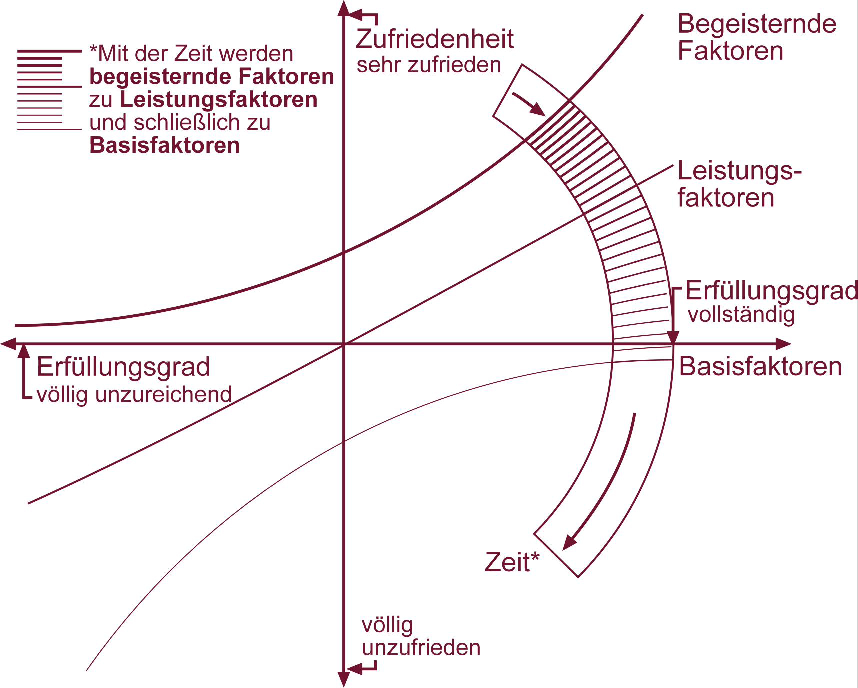
\includegraphics[width=.5\textwidth]{images/Kano-Modell.pdf}
\centering 
\captionabove[Das Kano-Modell]{Das Kano-Modell\footnotemark} 
\label{fig:kano}
\end{figure}
\footnotetext{Eine Darstellung des Kano-Modell (Quelle: \href{http://www.sophist.de/fileadmin/SOPHIST/Blog/Kano-Modell.jpg}{http://www.sophist.de/fileadmin/SOPHIST/Blog/Kano-Modell.jpg} Sichtung: 13.06.2017)} 

Doch was sind Basis-, Leistungs- und Begeisterungsfaktoren? Um ein Verständnis aufzubauen, werden diese im folgenden kurz erläutert.

\subsubsection{Basisfaktoren}
Basisfaktoren sind Features, welche von den Stakeholdern als selbstverständlich angesehen werden. Diese sollten in jedem Fall erfüllt werden, da sonst Unzufriedenheit der Kunden unvermeidbar ist. Wenn ein solches Feature fehlt, kann dies sogar dazu führen, dass ganze Stakeholder-Gruppen wegfallen.

\subsubsection{Leistungsfaktoren}
Leistungsfaktoren hingegen beschreiben Features, die bewusst von den Stakeholdern verlangt werden, jedoch nicht zwingend notwendig sind. Fehlen zu viele dieser Faktoren, hat auch das großen Einfluss auf die Zufriedenheit der Stakeholder. Wenn jedoch nur wenige dieser Faktoren fehlen, wird dies, im Gegensatz zu der Inakzeptanz bei den Leistungsfaktoren, meist geduldet und akzeptiert.

\subsubsection{Begeisterungsfaktoren}
Unter Begeisterungsfaktoren versteht man Features, welche der Kunde noch nicht kennt, deren Wert dem Nutzer allerdings während der Nutzung deutlich wird. Solche Faktoren heben das Produkt vom Markt ab und tragen erheblich zum Erfolg des Produkts bei. Meist stellen diese Faktoren ein Alleinstellungsmerkmal des Produktes dar. Doch setzt sich ein Begeisterungsfaktor auf dem Markt erst einmal durch, wird dieser nach nicht all zu langer Zeit von Stakeholdern oft als Leistungsfaktor oder sogar als Basisfaktor angesehen.\\

Ein gutes Beispiel dafür ist das Handy. Während früher mit einem Handy nur telefoniert werden konnte, hat sich irgendjemand ausgemalt wie es denn wäre, mit einem solchen Gerät auch Textnachrichten zu versenden. Dieses Feature war im ersten Moment ein Begeisterungsfaktor, denn die Nutzer kannten dieses Feature in dieser Form noch nicht. Im Laufe der Zeit haben sie es aber lieben gelernt. Kurze Zeit später wurde diese Funktion allerdings bei dem Kauf eines Handys bewusst verlangt, wodurch es dann von einem Begeisterungs- zu einem Leistungsfaktor wurde. Heute würde es sogar als Basis-Faktor eingestuft werden.

\section{Penalty-Reward-Faktoren Ansatz}
Ein anderer Ansatz Anforderungen schon bei der Ermittlung zu bewerten, ist der Penalty-Reward-Faktoren Ansatz. Hier geht es darum, die Dienstleistungsqualität einer Anforderung zu messen. Dazu werden den Anforderungen Penalty- und Reward-Faktoren zugeteilt. Penalty-Faktoren sind solche, die das Gesamturteil über ein System verschlechtern, allerdings bei einem Wegfallen auch nicht verbessern. Bei den Reward-Faktoren ist dies genau umgekehrt. Hier wird durch das Vorhandensein die Zufriedenheit der Stakeholder verbessert, das Wegfallen hat allerdings keine negative Auswirkung auf das Zielprodukt. Wie das aussehen kann, ist auf der Abbildung \ref{fig:penaltyreward} zu sehen.

\begin{figure}[!htb]
		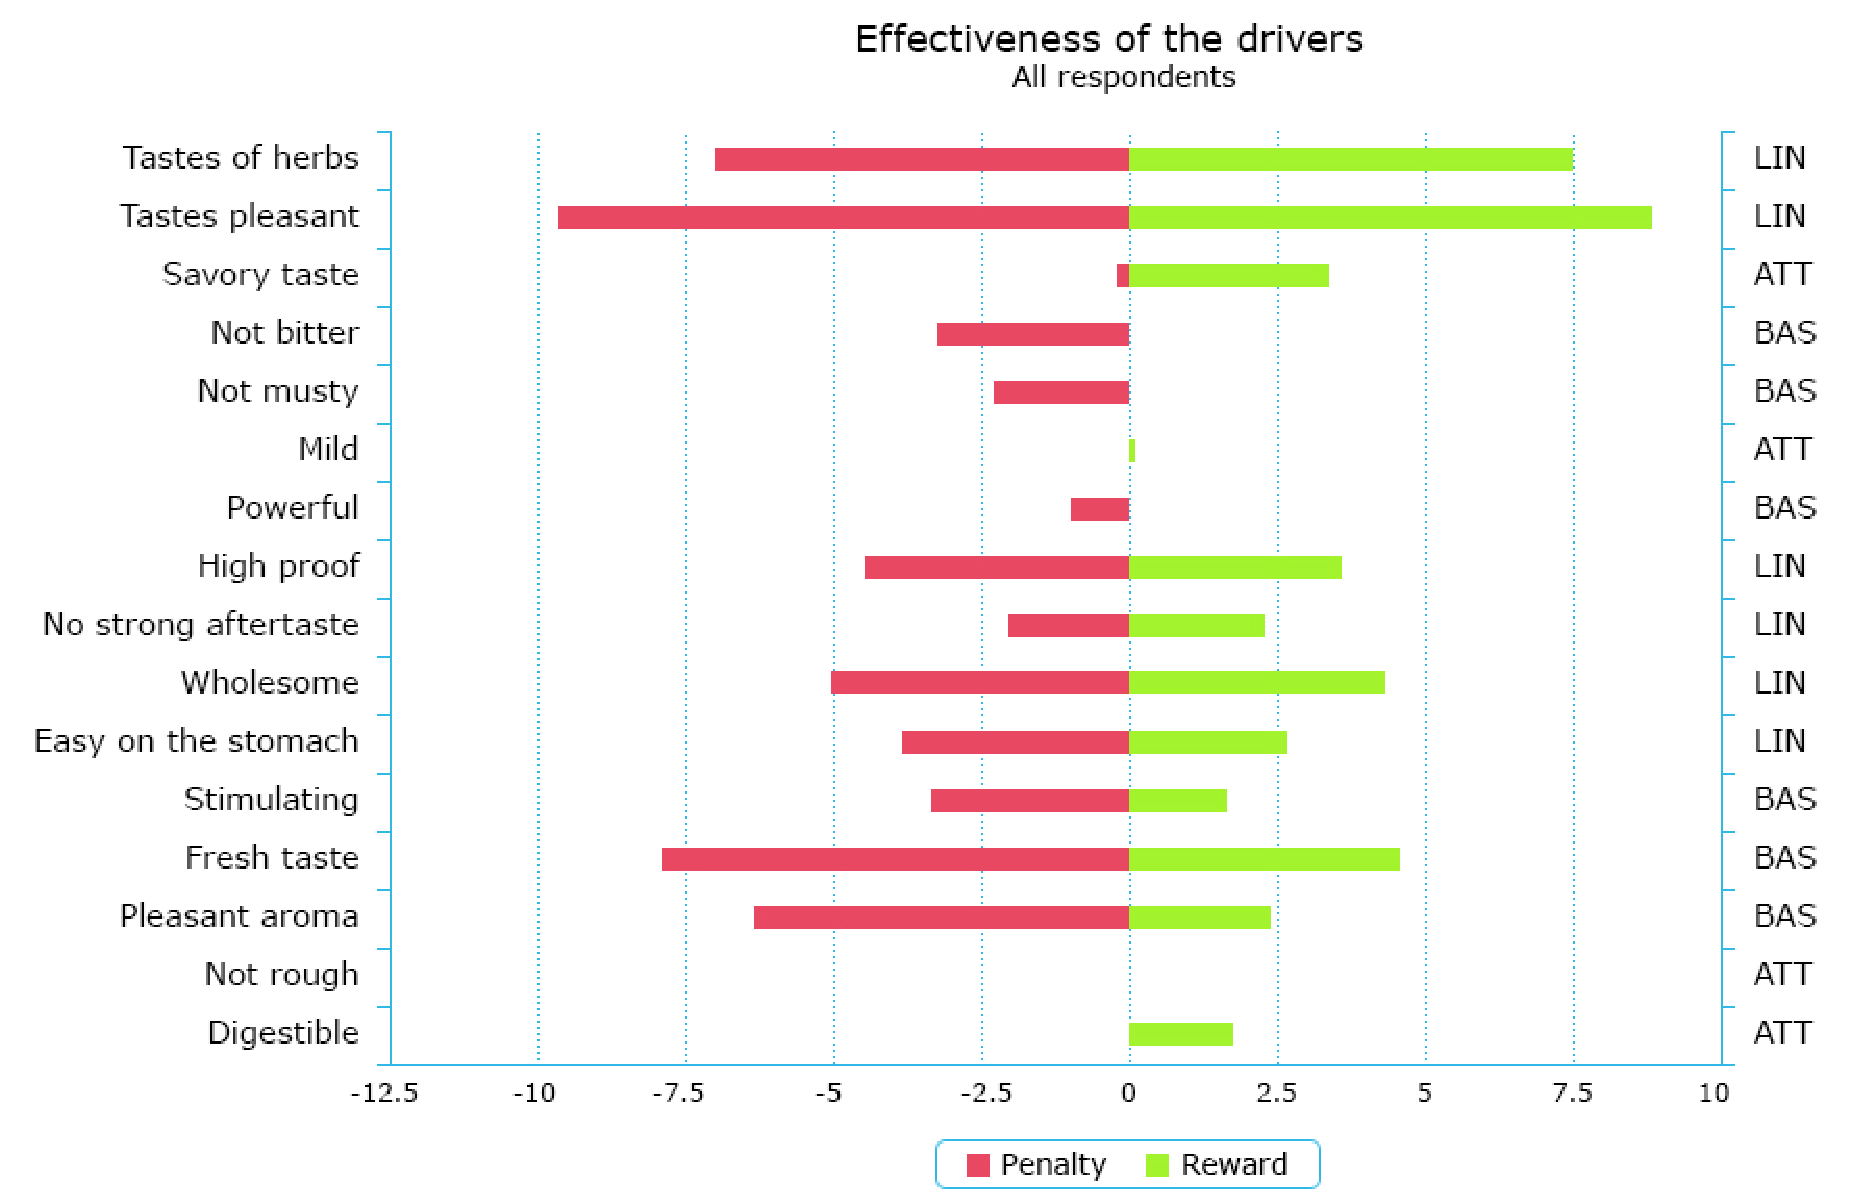
\includegraphics[width=\textwidth]{images/penaltyreward.pdf}
\centering 
\captionabove[Penalty-Reward-Analysis]{Penalty-Reward-Analysis\footnotemark} 
\label{fig:penaltyreward}
\end{figure}
\footnotetext{Eine Darstellung der Penalty-Reward-Analysis (Quelle: \href{https://www.ifad.de/services/multivariate-verfahren/neuere-ansaetze/penalty-reward-analyse-pra/?lang=en}{https://www.ifad.de/services/multivariate-verfahren/neuere-ansaetze/penalty-reward-analyse-pra/?lang=en} Sichtung: 13.06.2017)} 

\section{Anforderungen Ermitteln}
\label{subsec:ermittlung}
Wie kommt man jetzt an die Anforderungen der Stakeholder? \\
Vor der Ermittlung ist es wichtig, festzulegen, welche Art von Anforderungen man in Erfahrung bringen will. Während man bei einem \textit{"fertigen"} Produkt, möglicherweise nur neue Features und Ideen in Erfahrung bringen möchte, ist es bei einem Projekt in der Entwicklungs- oder Planungsphase durchaus wichtiger, vorerst die grundsätzlichen Wünsche und Anregungen der Stakeholder aufzunehmen. Dieser Schritt entscheidet, welche der vielen Methoden zur Ermittlung von Anforderungen eingesetzt wird. Welche Ermittlungs-Techniken es gibt, wurde von \cite{Rupp2} sehr gut und übersichtlich zusammengefasst, weshalb in dieser Arbeit nur auf den Kern dieser Methoden eingegangen wird. Grundsätzlich unterscheiden \cite{Rupp2} zwischen den Oberkategorien Kreativitäts-, Beobachtungs-, Befragungs- und artefaktbasierte Techniken. Was das ist, und wozu diese eingesetzt werden, zeigt die folgende Übersicht.

\subsection{Kreativitätstechniken}
\label{subsubsec:kreativitätstechniken}
Eine Art zur Ermittlung von Anforderungen sind Kreativitätstechniken. Diese werden eingesetzt, um neue innovative Ideen zu entwickeln. Hier versucht man aus dem herkömmlichen Denken auszubrechen, um die Tür für neue Ideen zu öffnen. Wichtig ist darauf zu achten, dass man sich vorher das richtige Umfeld schafft, um bessere Ergebnisse zu erzielen. Dann kann mit einer der folgenden Methoden der Kreativität freien Lauf gelassen werden.

\subsubsection{Brainstorming}
\label{subsubsec:brainstorming}
Die wohl bekannteste aller Kreativitätstechniken ist das Brainstorming. Dabei werden in einer Gruppe von fünf bis zehn Teilnehmern circa 20 Minuten Ideen gesammelt und vorerst ohne weitere Kommentare notiert. Anschließend werden diese Ideen sorgfältig analysiert. Durch diese Methode ist es möglich durch die Inspirationen durch Ideen anderer, eigene neue Ideen zu entwickeln.\\

Diese Technik bietet den Vorteil, dass viele Ideen in kurzer Zeit gefunden werden und die Teilnehmer diese zusammen6 entwickeln. Jedoch kann Brainstorming bei unterschiedlich dominanten Teilnehmern dazu führen, dass diese sich gegenseitig behindern. Auch ist diese Methode bei räumlich weit getrennten Stakeholdern problematisch.

\subsubsection{Brainstorming paradox}
Das Brainstorming paradox funktioniert fast genauso wie das normale Brainstorming, mit dem Unterschied, dass hier Ideen gesammelt werden, welche \textbf{nicht} erreicht werden sollen. Anschließend werden Maßnahmen entwickelt, welche diese Ideen vermeiden. \\

In manchen Situationen führt diese Methode schneller zu Ergebnissen. Auch werden so effektiv Risiken erkannt. Die Nachteile teilt sich diese Methode mit dem normalen Brainstorming.

\subsubsection{Methode 6-3-5}
Eine weitere Technik ist die Methode 6-3-5. Dabei handelt es sich um eine schriftliche Brainstorming-Methode. Hier bekommt jeder Teilnehmen einen Zettel, auf dem er innerhalb von circa fünf Minuten drei Ideen notiert. Anschließend wird dieser Zettel an den nächsten Teilnehmer weitergereicht, welcher, nachdem er die Ideen seines Kollegen durchgelesen hat, weitere drei Ideen hinzufügt. Dies wird solange wiederholt, bis jeder Teilnehmer einmal jeden Zettel hatte. Nach diesem Vorgang werden diese Ideen analysiert und zusammengefasst.\\

Da diese Technik schriftlich durchgeführt wird, lässt sie sich besonders bei einer komplizierteren Gruppendynamik einsetzen, da die in einer Diskussion aufkommenden Konflikte vermieden werden. Auch größere Distanzen zwischen den Stakeholdern können durch die Nutzung von Emails statt Zetteln bewältigt werden. Allerdings ist diese Methode, gerade durch die schriftliche Form und die zeitliche Begrenzung, nicht so effektiv wie das normale Brainstorming.

\subsubsection{Wechsel der Perspektive (6-Hut-Denken/Walt Disney-Methode)}
In manchen Situationen bietet es sich an, einen Wechsel der Perspektive vorzunehmen. Um dies zu erreichen gibt es viele verschiedene Techniken. Eine ausführliche Variante ist das \textit{6-Hut-Denken} von \textit{Edward de Bono} mit sechs Perspektiven. Diese kann man sowohl alleine als auch in Gruppen einsetzen. Die sechs Perspektiven lauten wie folgt:
\begin{enumerate}
  \setlength\itemsep{-4pt}
\item Objektivität und Neutralität
\item Persönliches Empfinden und subjektive Meinung
\item Objektive, negative Argumente
\item Objektive, positive Eigenschaften
\item Neue Ideen
\item Prozess-Kontrolle
\end{enumerate} 

Die Walt Disney-Methode ist benannt nach Walt Disney, der angeblich (so \cite{Rupp2}) für jede Sichtweise einen eigenen Raum hatte.
Hierbei wird der Stakeholder aufgefordert, jede der folgenden Perspektiven in einem anderen Raum oder zeitlich getrennt voneinander zu betrachten:

\begin{enumerate}
  \setlength\itemsep{-4pt}
\item Träumer und Visionär
\item Realist
\item Kritiker
\end{enumerate} 

Das Problem wird bei dieser Methode aus all diesen Perspektiven betrachtet, wodurch man einen sehr guten Überblick über das Gesamtbild des Projekts bekommt.\\

Mit diesen Techniken können auch Stakeholder, welche in ihrer Denkweise sehr festgefahren sind, veranlasst werden, die Dinge einmal aus einer anderen Perspektive zu betrachten. Jedoch ist es für viele schwierig sich in eine der genannten Rollen zu versetzen.

\subsubsection{Analogietechniken (Bionik/Bisoziation)}
Eine weitere Methode sind Analogietechniken. Bei einer Bionik werden als Denkmodell Analogie-Beispiele aus der Natur verwendet, um die dort gefundenen Lösungen auch auf das gegebene Problem anzuwenden. Um diesen Ansatz zu verstehen wird hier ein Beispiel von \cite{Rupp2} zitiert.

\begin{quote}
\textit{"Denken Sie zum Beispiel an die Fusion zweier Firmen und vergleichen Sie es mit dem Vermischen von zwei Tierherden. Wie lange dauert es, bis sich die Tiere der beiden Herden (die Mitarbeiter) vermischen? Die Leittiere werden in einen Konkurrenzkampf treten und eine neue Hierarchie erkämpfen. In einer Gefahrensituation, wenn zum Beispiel ein Raubtier die Herde angreift, werden sich die Tiere der beiden Tierherden als eine Herde verhalten, um ihre Chance zu verbessern, dem Raubtier zu entkommen. Diese Verhaltensmuster können in ähnlicher Form von den Mitarbeitern der beiden Firmen erwartet werden."}
\end{quote}

Bei der Bisoziation werden die Vorbilder im Gegensatz zu der Bionik nicht auf die Natur begrenzt.\\

Mit diesen Methoden ist es möglich, schwer vorstellbare Zusammenhänge oder komplexe Probleme durch den Kontextwechsel verständlich zu machen. Hierbei ist allerdings darauf zu achten, dass die verwendeten Vorbilder gut und passend ausgewählt werden. Dies nimmt unter Umständen viel Zeit in Anspruch.

\subsubsection{Osborn-Checkliste}
Die letzte der von \cite{Rupp2} aufgeführten Kreativitätstechniken ist die Osborn-Checkliste. Diese besteht aus den Punkten:
\begin{itemize}
\item Kann man das Produkt auch anders verwenden?
\item Gibt es etwas Ähnliches wie diese Produkt, und was können wir davon nachahmen?
\item Was lässt sich ändern? Kann man andere Funktionen einbauen?
\item Wie kann man das Produkt erweitern, veredeln oder teurer machen?
\item Wie kann man das Produkt vereinfachen oder auf Grundfunktionen reduzieren?
\item Kann man das Produkt oder Teile davon ersetzen?
\item Kann man das Produkt oder Teile davon umstellen, in der Reihenfolge verändern oder anders kombinieren?
\item Kann man auch das Gegenteil mit dem Produkt machen?
\item Kann man das Produkt oder die Idee mit etwas anderem kombinieren? Lässt es sich als Baustein für etwas anderes verwenden?
\item Kann man es in seiner Materie verändern? Kann man es zusammendrücken, verflüssigen, durchlöchern oder anders transformieren?
\end{itemize}

Durch die Beantwortung dieser Fragen, können gerade für ein bestehendes Produkt viele kreative Ideen gesammelt werden. Diese Methode für jede der Funktionalitäten eines großen Produkts anzuwenden kann allerdings zu aufwendig sein.

\subsection{Beobachtungstechniken}
Da aus verschiedenen Gründen nicht jeder Stakeholder in der Lage ist sein Know-how sprachlich auszudrücken, oder die Zeit hat dies zu tun, gibt es Beobachtungstechniken. Mit diesen Techniken werden Stakeholder beobachtet, um anhand ihrer Arbeitsabläufe neue Anforderungen zu entwickeln. Diese Methoden haben den Vorteil, dass sehr detaillierte Anforderungen aufgenommen werden können, da diese in der Regel von einem Fachmann selbst notiert werden.

\subsubsection{Feldbeobachtung}
Eine Beobachtungstechnik ist die Feldbeobachtung. Hierbei werden die Tätigkeiten und Arbeitsschritte der Stakeholder mit ihrem zeitlichen Zusammenhang erfasst. Unklare Arbeitsschritte können durch Fragestellungen an den Stakeholder geklärt werden.\\

Gerade für die Beobachtung unterbewusster Tätigkeiten eignet sich diese Methode sehr gut. Zudem können so leichter Abweichungen in den Prozessen analysiert werden, da der Requirements-Engineer viele Personen und ihre Tätigkeiten beobachtet. Jedoch gibt es Arbeitsabläufe die schwer bis gar nicht beobachtbar sind, diese können mit dieser Methode nicht ermittelt werden.

\subsubsection{Apprenticing}
Bei dieser Methode beobachtet der Requirements-Engineer den Stakeholder nicht, sondern erlernt die Tätigkeit, unter der Anleitung von diesem, selbst. So können die Anforderungen direkt aus der Perspektive des Stakeholders aufgenommen werden.\\

Im Gegensatz zur Feldbeobachtung fühlt sich der Stakeholder bei dieser Technik nicht beobachtet und unter Druck gesetzt. Auch bietet diese Methode psychologische Vorteile, weil der Requirements-Engineer selbst die Vor- und Nachteile eines Systems live aus der Sicht des Stakeholders erfährt.

\subsection{Befragungstechniken}
Befragungstechniken basieren darauf, Stakeholder gezielt nach ihren Wünschen und Bedürfnissen zu befragen. Für die Ermittlung von nicht-funktionalen Anforderungen ist diese Methode in den meisten Fällen nicht empfehlenswert, vielmehr wird diese dazu genutzt, funktionale Anforderungen aufzunehmen. Durch die Befragung können, je nach Umsetzung, viele neue Sichtweisen auf ein Problem erworben werden.

\subsubsection{Fragebogen}
\label{subsubsec:fragebogen}
Eine dieser Techniken ist der klassische Fragebogen. Hierfür werden eine Reihe von Fragen von den Stakeholdern, entweder online oder schriftlich, beantwortet. Diese Antworten werden anschließend ausgewertet um daraus Anforderungen zu entwickeln.\\

Mit dieser Methode kann eine große Anzahl von Stakeholdern eingebunden werden. Allerdings ist anzumerken, dass gerade implizites Wissen der Stakeholder untergeht. Auch können bei der Beantwortung dieser Fragen Unklarheiten schlecht geklärt werden, was zu einer Fehlinterpretation der Fragen führen kann.

\subsubsection{Interview}
\label{subsubsec:interview}
Bei einem Interview werden den Stakeholdern die Fragen im Gegensatz zu einem Fragebogen in einem direkten Gespräch gestellt und protokolliert. Auch hier werden diese anschließend ausgewertet und daraus Anforderungen entwickelt.\\

Der Vorteil dieser Methode ist, dass in einem offenen Gespräch oft die Hemmungen der Stakeholder gelindert werden. Des Weiteren kann der Verlauf des Gesprächs dynamisch angepasst werden. Mit dieser Technik kann besonders das Qualitätskriterium der Vollständigkeit leichter erfüllt werden als mit anderen Techniken. Jedoch sind solche Interviews sehr zeitaufwendig, was das Befragen vieler Stakeholder in den meisten Fällen erschwert.

\subsubsection{Selbstaufschreibung}
Eine weitere Form der Befragung ist die Selbstaufschreibung. Bei dieser Methode beschreibt der Stakeholder selbst Anforderungen, Änderungs- und Optimierungsvorschläge an das System. Die Qualität der Ergebnisse kann verbessert werden, indem die ausgewählten Stakeholder in die Grundlagen der Anforderungsanalyse eingewiesen werden.

Durch die Selbstaufschreibung wird der Stakeholder nicht von dem Requirements-Engineer beeinflusst. Zudem muss er sein Wissen nicht erläutern, sondern nutzt eine gleichbleibende Formulierung für seine Anforderungen.

\subsubsection{On-Site-Customer}
Anders als bei vielen anderen Methoden ist bei On-Site-Customer ein Interessenvertreter der Stakeholder während der Entwicklung ständig vor Ort. So können, besonders in einzelnen Inkrementen, die Anforderungen und deren Umsetzung optimiert werden.\\

Anforderungen werden so vor allem mündlich und sehr schnell ermittelt, dennoch ist es für viele schwierig, einen geeigneten Mitarbeiter für solche Zwecke dauerhaft zu entbehren. Auch werden bei einer fehlenden Abstimmung zwischen dem On-Site-Customer und den anderen Stakeholdern nur die Interessen einer Person vertreten.\\[1em]

\cite{Rupp2} beschreiben darüber hinaus noch Artefaktbasierte- und unterstützende Techniken zur Ermittlung von Anforderungen. Diese beziehen sich größtenteils nicht auf die Stakeholder, sondern auf existierende Systeme oder andere Quellen. Diese Art der Anforderungsermittlung entspricht nicht dem eigentlichen Sinn dieser Arbeit, weshalb diese auch nicht weiter erläutert werden.

\section{Dokumentation}
\label{subsec:dokumentation}
Um Anforderungen nach der Ermittlung bestmöglich verarbeiten zu können, ist es notwendig, diese in einem einheitlichen und fachlichen Stil zu dokumentieren. Auch hier finden sich viele Techniken dies zu tun. Einen Überblick über die wichtigsten dieser Techniken geben die folgenden Abschnitte.

\subsection{User-Storys}
Eine Möglichkeit Anforderungen zu dokumentieren sind User-Storys. Einzelne Systemfunktionalitäten werden in kleine Storys verpackt, welche aus der Sicht des Users formuliert sind. Diese dienen in wenigen Sätzen als Gedankenstütze zu der Anforderung. Eine User-Story könnte wie folgt lauten:

\begin{quote}
\textit{"Als Mitarbeiter möchte ich Urlaub vorab über ein elektronisches Formular beantragen können, damit ich eine offizielle Genehmigung erhalte um dann eine Ferienreise verbindlich buchen zu können."}
\end{quote}

User-Storys bilden zwar neben der eigentlichen Anforderung auch die Intention des Users ab, jedoch sind diese teilweise für die Entwickler schwieriger zu implementieren, da sie meist dafür zu grob formuliert sind.

\subsection{Use-Cases}
Ähnlich wie bei User-Storys bilden Use-Cases die Anforderung aus der Sicht des Users ab, diese sind aber in den meisten Fällen wesentlich grober formuliert. Auch werden hier oft sogar nur einzelne Aktionen beschrieben. Einige Beispiele dazu könnten lauten:
\begin{quote}
\textit{"Geld abheben"}
\textit{"Überweisung tätigen"} oder
\textit{"Kontostand überprüfen"}
\end{quote}

\subsection{Technical Storys}
Da Anforderungen nicht immer nur Funktionalitäten beschreiben, sondern manchmal auch technische Details, können diese gegebenenfalls nicht in User-Storys beschreiben werden. Um diese dennoch zu betrachten, werden Technical Storys verwendet. Diese sind im Prinzip nichts anderes als User-Storys, welche aus technischer Sicht eine nicht-funktionale Anforderung beschreiben.

\subsection{FunctionsMASTeR}
\label{subsec:functionmaster}
Eine weitere Alternative zur Dokumentation von Anforderungen beschrieben \cite{SOPHIST2}. Hierbei dient eine ganz einfach Schablone dazu, die wichtigsten Informationen einer Anforderung in einen Satz zu verpacken. Diese Schablone sieht wie folgt aus:

\textit{<System> <muss,sollte,wird>} \textit{<Akteur>, fähig sein} \textit{<Objekt> <Prozesswort>}\\

Diese Methode hat den Vorteil, dass so nicht nur funktionale, sondern auch nicht-funktionale Anforderungen, dokumentiert werden können. Auch ist diese Form der Beschreibung für die Entwickler gut interpretierbar.

\section{Validation}
Die Validation ist ein wichtiger Schritt im \acl{RE}. Nachdem die Anforderungen dokumentiert wurden muss geprüft werden, ob diese auch tatsächlich umsetzbar sind. Es kann vorkommen, dass Anforderungen über den Funktionsrahmen des Systems hinaus gehen und somit vorerst nicht mehr in Betracht gezogen werden. Dieser Schritt stellt also eine Überprüfung aller Anforderungen dar, wobei nicht valide Anforderungen aussortiert werden. Dies kann in Zusammenarbeit mit dem Entwickler-Team oder dem Product-Owner geschehen.  

\section{Auswertung}
Die ermittelten Anforderungen müssen vor der eigentlichen Implementierungsarbeit ausgewertet werden. Das sorgt für eine detailliertere Priorisierung. So kann ein Plan erstellt werden, ob und in welcher Reihenfolge diese erfüllt werden. Die bekanntesten Methoden eine Auswertung durchzuführen werden im folgenden Abschnitt kurz erklärt.

\subsection{Function-Point-Analyse}
Mit der \ac{FPA} wird der Aufwand einzelner Anforderungen oder Anforderungsgruppen gemessen. Dieser Aufwand wird in Function-Points angegeben. Bei dieser Methode werden (so \cite{Lipinski}) in drei Stufen die sogenannten unbewerteten oder auch unjustierten \ac{FP} bestimmt. Dazu werden in der ersten Stufe Parameter wie: Anzahl der Benutzer- Eingaben und Ausgaben, Anzahl der Benutzerabfragen, Anzahl der Datenbankspalten und die Anzahl der Schnittstellen zu externen Systemen in die Berechnung mit einbezogen. Die so errechneten \ac{FP} werden anschließend in der zweiten und dritten Stufe durch Komplexitätsparameter und Konstanten des Entwicklungsprozesses gewichtet. Anschließend werden den Anforderungen Werte für bestimmte Charakteristika, wie die Wiederverwertbarkeit, zugewiesen. \\

Nach diesen drei Stufen spricht man von bewerteten oder auch justierten \ac{FP}. Diese werden, um eine Aussage über den Implementierungsaufwand treffen zu können, anschließend mit Erfahrungswerten und der Produktivität von Software-Entwicklungsprozessen verglichen und in Mitarbeiter-Monate umgerechnet. Mitarbeiter-Monate geben an, wie viele Monate ein Mitarbeiter für die Umsetzung benötigt.\\

Diese Methode beruht zwar im Gegensatz zu anderen Methoden größtenteils nicht auf Schätzungen sondern auf Fakten und Erfahrungswerten, jedoch ist die Ermittlung des Aufwands mit dieser Technik sehr zeitaufwendig und komplex. Auch zeigt laut der \cite{AGIL1} die Erfahrung, dass das vergleichende Schätzen, wie es bei Story-Points durchgeführt wird, zu deutlich schnelleren und besseren Ergebnissen führt.

\subsection{Story-Points}
Eine Aufwandsschätzung mit Story-Points ist wesentlich schneller als der langwierige Prozess der Function-Point-Analyse und stellt deshalb vor allem in agilen Projekten eine gern gesehene Alternative dar. Hierzu werden den zuvor erstellten User-Storys Story-Points zugewiesen, welche eine abstrakte Komplexität der einzelnen Storys angibt. Dabei wird eine Skala festgelegt, in welcher die Story-Points vergeben werden. \cite{Preuss1} empfiehlt als Skala eine abgeänderte Form der Fibonacci-Folge zu verwenden, welche aus den Elementen 1, 2, 3, 5, 8, 13, 20, 40 und 100 besteht. User-Storys mit vielen Story-Points bedeuten, dass diese Story in kleinere Storys aufgeteilt werden muss, um realistisch abgeschätzt werden zu können. Man kann allerdings auch eine einfache Skala von beispielsweise 1-10 nutzen.\\

Nach der Festlegung dieser Skala wird eine Story ausgesucht, die einen guten Mittelwert an Komplexität mit sich bringt. An dieser Story wird sich bei der Vergabe weiterer Story-Points orientiert. \\[1em]

Es gibt noch weitere Methoden zur Aufwandsschätzung einer Anforderung, wie beispielsweise das CoCoMo (mehr dazu auf \cite{COCOMO}), die COSMIC-Methode der \cite{COSMIC}, Lines of Code, Ad-hoc-Schätzmethoden oder umfangbasierte Schätzmethoden. Eine gute Übersicht über diese Methoden bietet das \cite{WinfWiki}.


%======================================================================
%======================================================================
% Eintrag ins Glossar
\nomenclature{Requirement-Engineering}{Der Prozess der Ermittlung, Analyse, Auswertung und Bearbeitung von Anforderungen.\vspace{4mm}}

\nomenclature{Requirement-Engineer}{Die Person, welche das Requirement-Engineering durchführt.\vspace{4mm}}

\nomenclature{System}{System wird im Kontext dieser Arbeit als Synonym für das zu entwickelnde System eingesetzt.\vspace{4mm}}

\nomenclature{Produkt}{Ein weiteres Synonym für das zu entwickelnde System.\vspace{4mm}}

\nomenclature{Projekt}{Der Prozess zur Planung und Entwicklung eines Systems.\vspace{4mm}}

\nomenclature{Usability}{Das Ausmaß, in dem ein Produkt durch bestimmte Benutzer in einem Nutzungskontext benutzt werden kann, um ein Ziel effektiv, effizient und zufriedenstellend zu erreichen.\vspace{4mm}}

\nomenclature{Funktion-Points}{Ein Maß für den Aufwand der Umsetzung einer Funktionalität. Diese finden Anwendung in der Function-Point-Analyse\vspace{4mm}}

\nomenclature{User-Story}{Eine Art Anforderungen aus der Sicht des Nutzer zu dokumentieren.\vspace{4mm}}

\nomenclature{Story-Points}{Ein Maß zur Angabe der Komplexität einer User-Story.\vspace{4mm}}

\nomenclature{Use-Cases}{Eine Art Funktionalitäten die ein System bieten soll zu beschreiben.\vspace{4mm}}

\nomenclature{User}{Der Nutzer eines Systems.\vspace{4mm}}

\nomenclature{Potentieller Nutzer}{Ein möglicher zukünftiger Nutzer eines Systems.\vspace{4mm}}
	
	% Die Zähler für Tabellen und Abbildungen werden zurückgesetzt, damit
	% in jedem Kapitel die Nummerierung neu beginnt
\setcounter{table}{1}
\setcounter{figure}{1}
	% Einbinden des dritten Kapitels
	%!TEX root = ../draft.tex
\chapter{Umsetzung}
Das Anforderungsmanagement teilt sich in mehrere Abschnitte ein, jeder dieser Abschnitte stellt einen wichtigen Prozess für den Umgang mit Anforderungen dar. Der erste Schritt ist die \nameref{sec:ermittlung}, wobei die Anforderungen der Stakeholder ermittelt werden, um sie daraufhin zu dokumentieren. Ist die \nameref{sec:dokumentation} abgeschlossen, folgt die \nameref{sec:auswertung} der dokumentierten Anforderungen. Bei einem agilen Projekt wie es das \ac{LWM} darstellt, wird dieser Vorgang in Iterationen bis zu einem beliebigen Detailgrad immer wieder verfeinert.

\section{Ermittlung}
\label{sec:ermittlung}

Aus der Problemstellung ist zu entnehmen, dass nicht das Ermitteln neuer ausgefallener Ideen und Features das Ziel ist, sondern das in Erfahrung bringen der Wünsche und Voraussetzungen der Stakeholder. In anderen Worten: Es wird das Ziel verfolgt Basis- und Leistungsfaktoren zu ermitteln. Aus diesem Grund wurde bewusst Abstand von den in Kapitel \ref{subsubsec:kreativitätstechniken} beschriebenen Kreativitätstechniken genommen. Auch wurde sich gegen die in Kapitel \ref{subsubsec:fragebogen} aufgeführten Fragebogen-Methode entschieden, da die befragten Stakeholder dazu nicht über genügende Kenntnisse über das Produkt verfügten.\\

Unter anderem aus diesem Grund, etablierte sich die \nameref{subsubsec:interview}-Technik. Bei dieser Technik geht es darum, ein Interview über vorbereitete und vorformulierte Fragen mit den gewählten Stakeholdern zu führen. So ist es möglich, während dem Gespräch auftretende Fragen direkt zu klären und somit auch implizite Anforderungen aufzudecken. Zudem öffnet diese Methode die Tür für neue Anforderungen oder Problemstellungen, welche bislang nicht in Betracht gezogen wurden. 
Ein weiterer Vorteil dieser Technik ist, dass die Hemmungen der Stakeholder durch ein offenes Gespräch gelindert werden.\\

Zu Beginn der Ermittlung wurde ein zweiseitiger Fragebogen (siehe Anhang \ref{anh:fragebogen}) als Leitfaden für die Interviews erstellt, welcher in kurzen Stichpunkten die wesentlichen Problemstellungen und Platz für die darauf bezogenen Notizen beinhaltet. Die dort aufgeführten Probleme beruhen auf Erfahrungen mit dem bestehenden Tool und wurden durch  \nameref{subsubsec:brainstorming} ergänzt. 
Mit diesem Formular konnte nicht nur der Umgang mit den bekannten Problemen des Tools, sondern auch solche, die aus Ausnahmesituationen resultieren, zur Sprache gebracht werden.\\

Im Anschluss daran wurde mit Hilfe des Entwickler-Teams, sowohl Frontend als auch Backend, eine Eingrenzung der Stakeholder vorgenommen. Dieser ausgewählte Kreis wurde per E-Mail kontaktiert und um einen Gesprächstermin gebeten, sofern Interesse an der Nutzung eines Tools zu Verwaltung der Praktika besteht. \\

Bei dem Ablauf der Interviews ist grundsätzlich zwischen den aktuellen Nutzern und den potentiell zukünftigen Nutzern zu unterscheiden. Zwar wurde das Ziel verfolgt, losgelöst von dem aktuellen Tool über ein "Wunschsystem" zu sprechen, jedoch war dies einerseits bei den bestehenden Nutzern kaum möglich, da diese sich instinktiv immer wieder an dem derzeitigen Tool orientierten. Andererseits konnte dieses bei den Stakeholdern, für die dieses System zu diesem Zeitpunkt noch unbekannt war, als perfekte Beschreibung der Thematik genutzt werden.\\

Ein Interview begann, sofern erforderlich, mit der Beschreibung des bestehenden Tools, um eine Ausgangsgrundlage für das Gespräch zu schaffen. Nach der Darlegung der Problemstellung war jedem Gesprächspartner der Hintergrund dieser Anforderungsermittlung bekannt. Mit der Aufforderung, zunächst vollkommen losgelöst von den vorgefertigten Fragen, den Ablauf des Praktikums und dessen Bewertung zu erklären, konnten zu diesem Zeitpunkt schon eine Vielzahl dieser Fragen beantwortet werden. Diese Informationen wurden durch Fragen mit einem "Was wäre wenn"-Stil ergänzt, wobei zu beachten war, dass die Gesprächspartner nicht in eine vorgegebene Denkweise geleitet werden. So wurden auch kleinste Probleme, die bei der Nutzung eines solchen Tools auftreten können, aufgedeckt und dokumentiert.\\

Die Anforderungen der Nutzer wurden während des Gesprächs bestmöglich in die Kano-Faktoren eingeteilt, welche in Kapitel \ref{sec:kano} beschrieben wurden. Dadurch konnte eine grobe Priorisierung nach \textit{Basisfaktoren}, \textit{Leistungsfaktoren} und \textit{Begeisterungsfaktoren} schon vor der eigentlichen Auswertung vorgenommen werden.\\

Durch die Interviews konnten über 150 Anforderungen ermittelt werden, wovon einige durch das gegenwärtige Tool schon abgedeckt werden und andere, welche eine ganz neue Perspektive auf das System und dessen Möglichkeiten ermöglichen.


\section{Zielgruppe}

Als Stakeholder ist grundsätzlich jeder zu betrachten, der aktiv an dem Tool oder dessen Nutzung beteiligt ist oder durch diese beeinflusst wird. Durch diese Definition befinden sich in der Gruppe der Stakeholder nicht nur das Entwickler-Team, sondern auch Studenten, Administratoren, Modulverantwortliche, Mitarbeiter, \ac{SHK} und \ac{WHK}. \\[1em]

Die Anforderungsermittlung über Studenten wurde nicht in Betracht gezogen, da dies nicht in den zeitlichen Rahmen dieser Arbeit gepasst hätte. Zudem sind Studenten zwar direkte Nutzer des Systems, jedoch arbeiten sie, im Gegensatz zu den anderen Stakeholdern, verhältnismäßig wenig damit.\\
Die Anforderungen des Entwickler-Teams wurden, im Laufe der Anforderungsauswertung  und Validation, aufgenommen.\\
Von den verbleibenden Stakeholdern erwies es sich als sinnvoll, die Modulverantwortlichen als Interessenvertreter anzusehen.\\[1em]

Durch das Modulhandbuch des Campus konnte eine Liste der existierenden Module erstellt werden. Die Email-Adressen der Modulverantwortlichen konnte von der Webseite der TH-Köln bezogen werden.\\
Mit der Vorgabe den Kreis der Nutzer auf den Bereich des Instituts für Informatik zu begrenzen, beinhaltet diese Liste 61 Module.\\

Durch ein Gespräch mit dem Entwickler-Team, konnte diese Liste anschließend auf circa 20 Module begrenzt werden, indem die Module, die kein Praktikum veranstalten, aussortiert wurden.\\

Nach der Kontaktierung der jeweiligen Modulverantwortlichen, bestätigten 14 von diesen ein Interesse an diesem Projekt und erklärten sich zu einem Interview bereit.

\section{Dokumentation}
\label{sec:dokumentation}

\subsection{Formulierung}

Um die auf den Interview-Bögen notierten Anforderungen, mit allen nötigen Details, zu dokumentieren, wurde auf eine abgewandelte Form der in Kapitel \ref{subsec:functionmaster} erläuterten Schablone zurückgegriffen. \\

In einer etwas angepassten Form sieht der Satzbau wie folgt aus:\\

\textit{<Zielsystem> <Priorität>} einem \textit{<Stakeholder>} die Möglichkeit bieten, \textit{<Funktion>}.\\

Erklärung:
\begin{description}
\item \textit{<Zielsystem>}

Das Zielsystem stellt das referenzierte System dar. Hierbei steht \textit{"Das bestehende System"} für das aktuelle \ac{LWM} und \textit{"Das zu entwickelnde System"} für ein neues System . Die Unterscheidungen dieser Systeme wird in Kapitel \ref{sec:auswertung} genauer erläutert. 

\item \textit{<Priorität>}

Hier wird mit Hilfe des Kano-Modell von Prof. Noriaki Kano priorisiert. Für einen Basis-Faktor wird, mit Anlehnung an \cite{Rupp14}, das Schlüsselwort \textit{"muss"}, für einen Leistungs-Faktor \textit{"soll"} und für einen Begeisterungsfaktor \textit{"wird"} eingesetzt. 

\item \textit{<Stakeholder>}

Hier wird die Liste von Stakeholdern, welche von dieser Anforderung Gebrauch machen würden eingesetzt.

\item \textit{<Funktion>}

Die Funktion beschreibt den eigentlichen Sinn dieser Anforderung.

\end{description}

Ein Beispiel aus dieser Arbeit sieht wie folgt aus:\\

\textit{"Das bestehende System soll einem Modulverantwortlichen und einem Mitarbeiter die Möglichkeit geben, eine gelbe Karte für eine unbefriedigende Abgabe zu erteilen."}\\

oder:\\

\textit{"Das zu entwickelnde System wird einem Modulverantwortlichen, einem Mitarbeiter, einer Studentischen Hilfskraft und einem Studenten die Möglichkeit geben, Termine in einer gegebenen Frist zu stornieren."}

\section{Auswertung}
\label{sec:auswertung}

Für die Arbeit mit den Anforderungen, ist es notwendig, diese auszuwerten.
Das \ac{LWM} ist ein agiles Projekt, weshalb es sinnvoll war, auch die Anforderungsauswertung diesem Stil entsprechend durchzuführen. Hierzu wurden die Anforderungen nach der \nameref{subsec:validation} in einer Art Epic zusammengefasst. Anschließend wurden diese Gruppen priorisiert. Hier setzt ein neuer Iterationsschritt ein, indem eine Gruppe mit der höchsten Priorität selektiert und wiederum in Untergruppen eingeteilt wurde. Diese Untergruppen konnten anschließend wieder priorisiert werden. Dieser Vorgang kann je nach Belieben wiederholt werden. Ist der gewünschte Detailgrad erreicht, fällt es leicht die Komplexität der einzelnen Anforderungen zu schätzen.


\subsection{Validation}
\label{subsec:validation}
Der erste Schritt in der Auswertung war die Validation. Die Anforderungen wurden für ein schon bestehendes System aufgenommen, weshalb es vorkommen kann, dass Anforderungen schon erfüllt wurden. Um die spätere Verarbeitung zu vereinfachen, wurde deshalb im Vorfeld eine Validation der Anforderungen vorgenommen. Hierbei wurden diese in drei Kategorien aufgeteilt. Es wurde unterschieden zwischen \textit{"Erledigt"}, \textit{"Valide"} und \textit{"Verworfen"}. Die Anforderungen aus den Kategorien \textit{"Erledigt"} und \textit{"Verworfen"} werden zwar nicht gelöscht, da diese auch während der Implementierung von anderen Anforderungen von Relevanz sein können, jedoch werden diese bei der Priorisierung nicht beachtet. Auch gibt es für diese Anforderungen im ersten Moment keine Aufwandsschätzung, da diese derzeit keinen Aufwand bedeuten.

\subsection{Gruppierung}

Eine unsortierte Liste von Anforderungen kann nicht so einfach ausgewertet werden, weshalb ein Verfahren gefunden werden muss, diese Anforderungen in kleinere Gruppen zu sortieren. Mit diesen Gruppen fällt nicht nur die Übersicht leichter, sondern auch die spätere Priorisierung und Aufwandsschätzung.\\

Im Laufe der Anforderungsermittlung wurde deutlich, dass einige Anforderungen die eigentliche Grenze des aktuellen \ac{LWM} überschreiten. So wurde beispielsweise ein Forum für das Besprechen von Problemstellungen gefordert, was jedoch nicht direkt mit der Praktikumsverwaltung selbst zu tun hat. Da diese Ideen jedoch nicht verworfen werden sollen, da sie einen Mehrwert für den Praktikumsverlauf darstellen, wurde mit dem Entwickler-Team die Entscheidung getroffen, die Anforderungen aufzuteilen. Die erste Gruppierung erfolgte somit durch die Unterscheidung, ob eine Anforderung einem neuen System, oder dem bestehenden System zuzuordnen ist.\\

Des Weiteren wurde sich für eine Gruppierung nach Aufgabengebiet entschieden. Dies ist ein sehr grobes Verfahren, was allerdings in Anbetracht der Menge von Anforderungen, als angemessen empfunden wurde. Ganz nach dem Prinzip \texttt{divide and conquer} wurden erst wenige große Gruppen erstellt, die anschließend durch weitere Iterationen verfeinert werden. \\

Eine Möglichkeit Anforderungen in einer höheren Abstraktionsebene zu beschreiben sind Epics. Epics beschreiben eine Masse an Anforderungen mit einer User-Story. Auch wenn das Prinzip von Epics in diesem Anwendungsfall verfolgt wurde, fiel die Entscheidung gegen die Beschreibung in Form einer User-Story, da dies auf diesem Abstraktionslevel nicht angebracht war. Ab einem gewissen Detailgrad ist dies jedoch durchaus sinnvoll.\\

Diese Gruppierung erfolgte durch die Aufteilung in Aufgabengebiete an einem Whiteboard. 
\begin{figure}[!htb]
		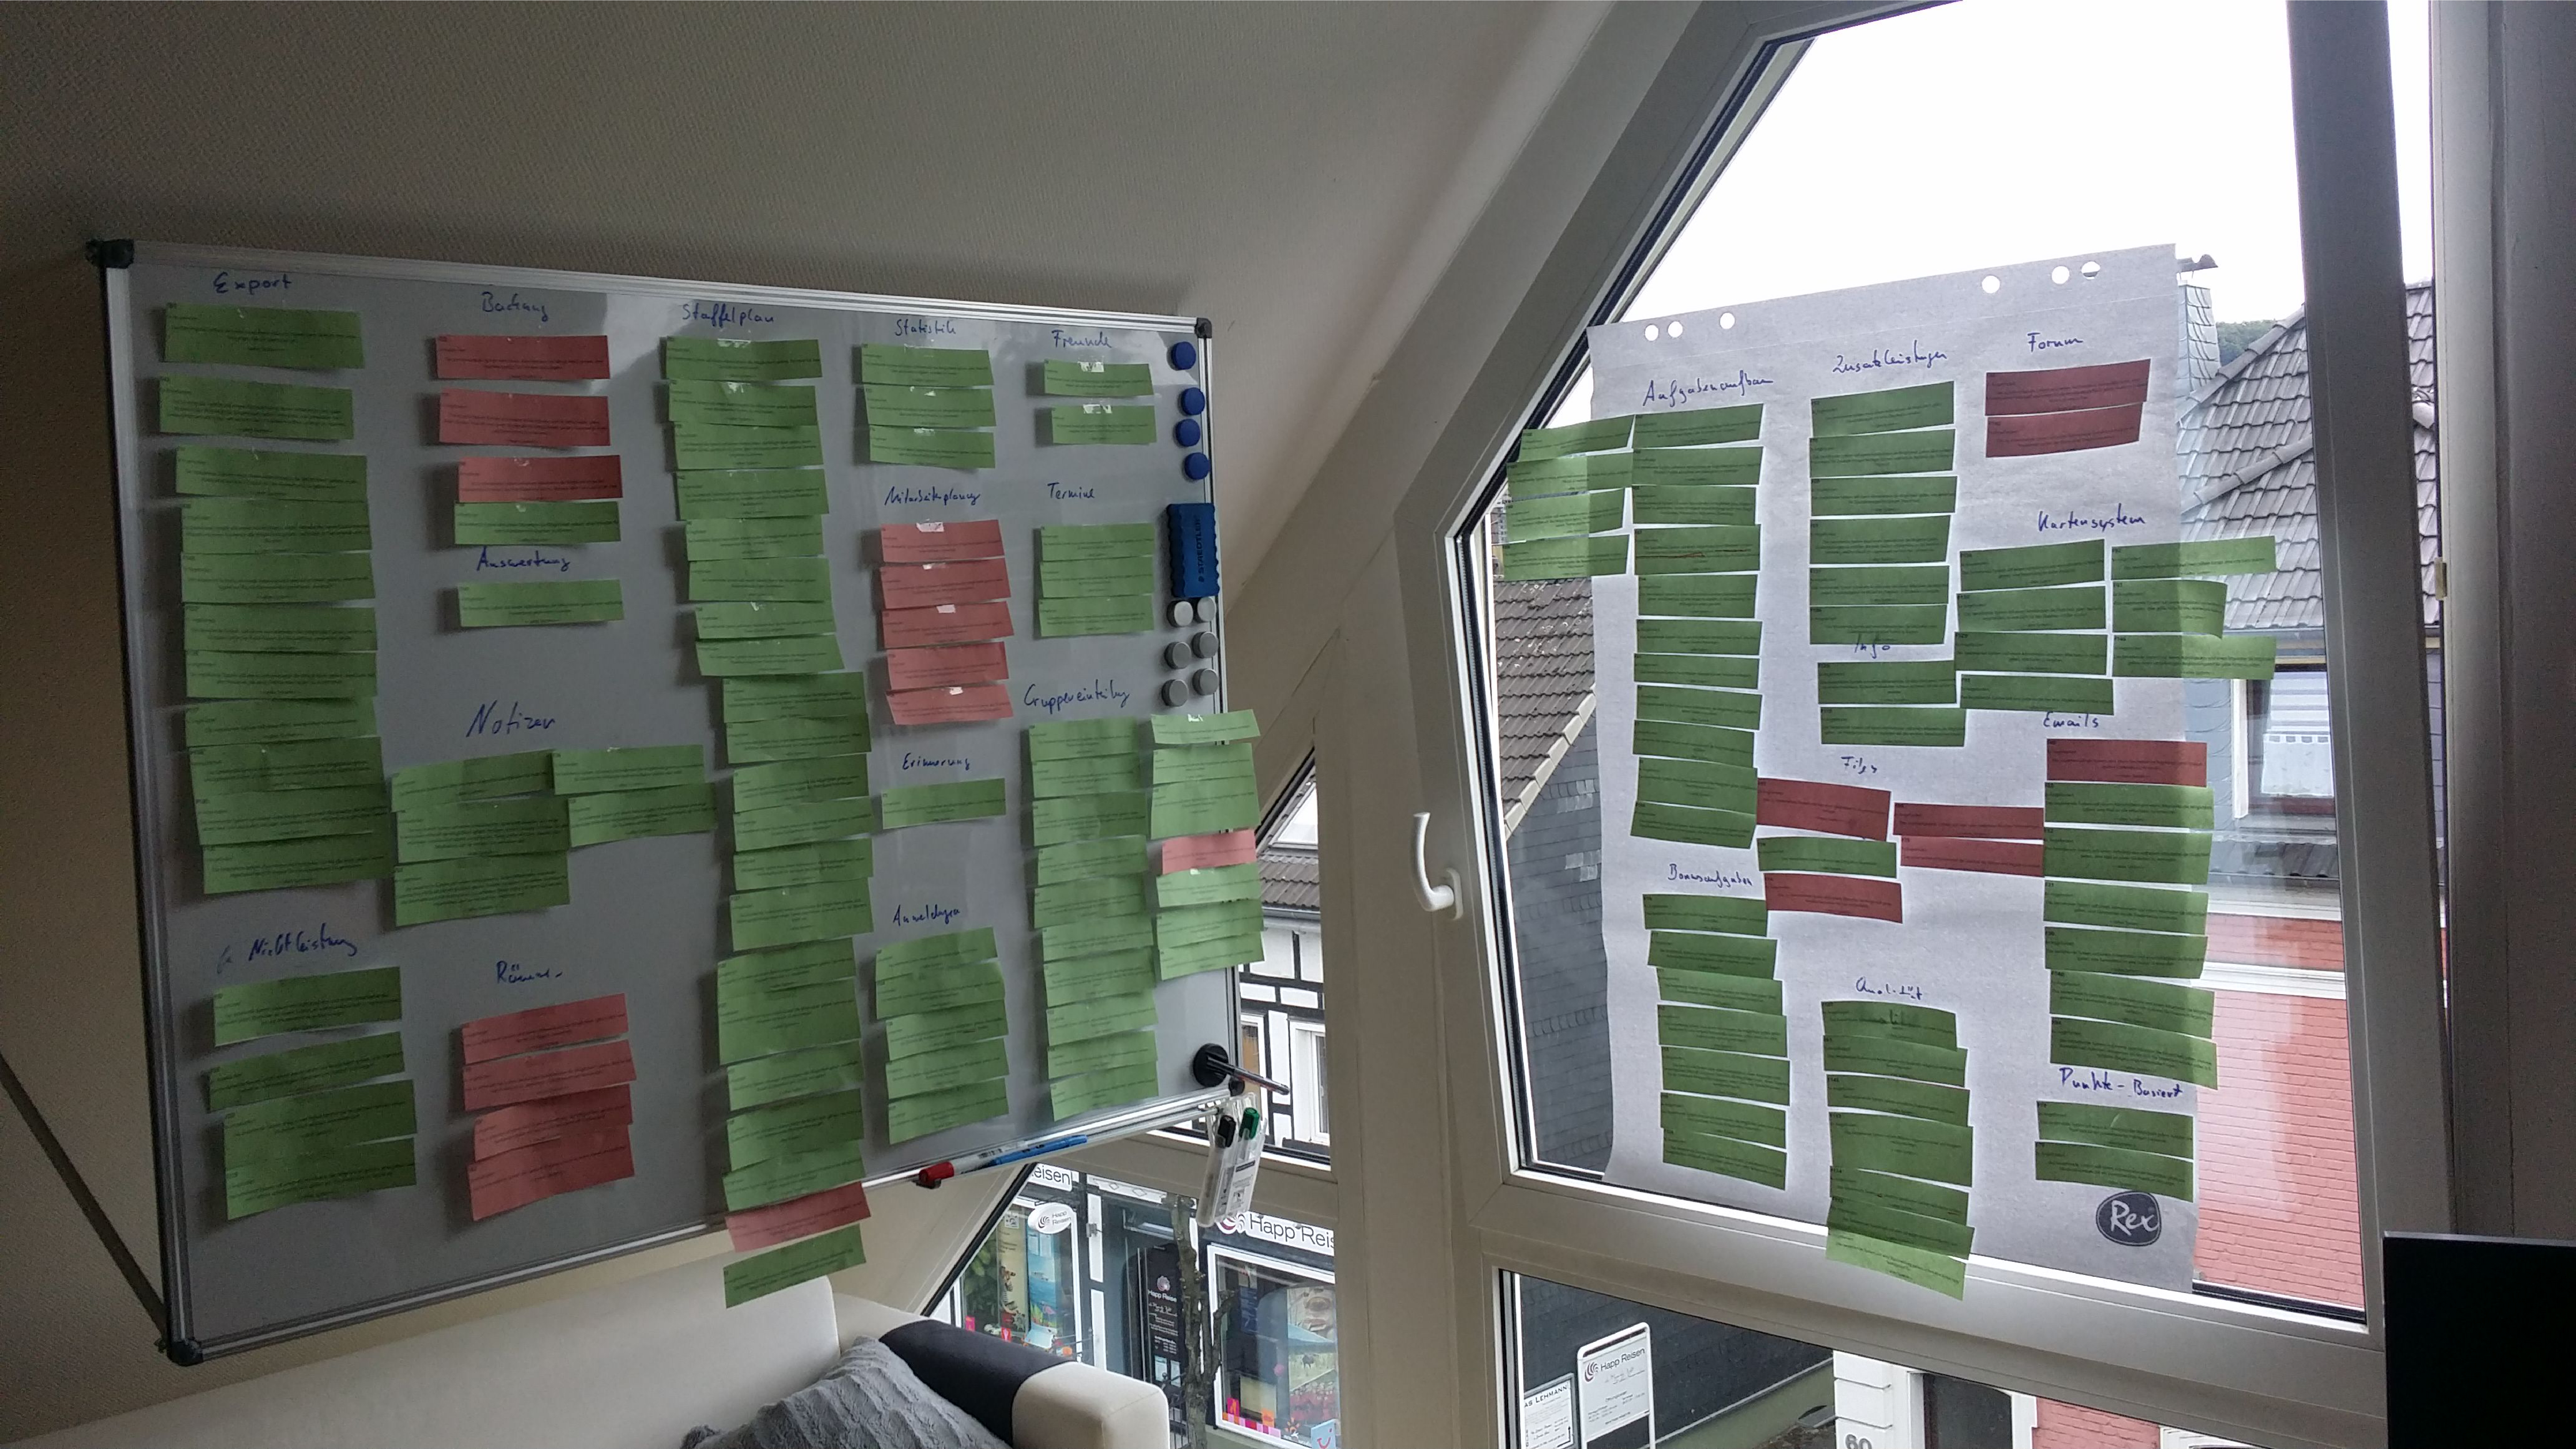
\includegraphics[width=\textwidth]{images/erstegruppen.pdf}
\centering 
\captionabove[Gruppeneinteilung zweiter Ebene]{Gruppeneinteilung zweiter Ebene\footnotemark} 
\end{figure}
\footnotetext{Ein Bild von der Gruppeneinteilung auf zweiter Ebene an einem Whiteboard} 

So konnten die circa 150 Anforderungen in 24 Gruppen eingeteilt werden.\\

Nach der ersten Priorisierung, auf welche in Kapitel \ref{subsec:priorisierung} näher eingegangen wird, wurde zunächst die Gruppe mit der höchsten Priorität ausgewählt, um sie in kleinere Einheiten zu zerlegen. Dies erfolgte in einem Meeting gemeinsam mit dem Entwickler-Team. Hierzu wurden die Anforderungen der Gruppe \textit{"Staffelplan"} auf einem Whiteboard in eine Ablaufreihenfolge gebracht. 

\begin{figure}[!htb]
		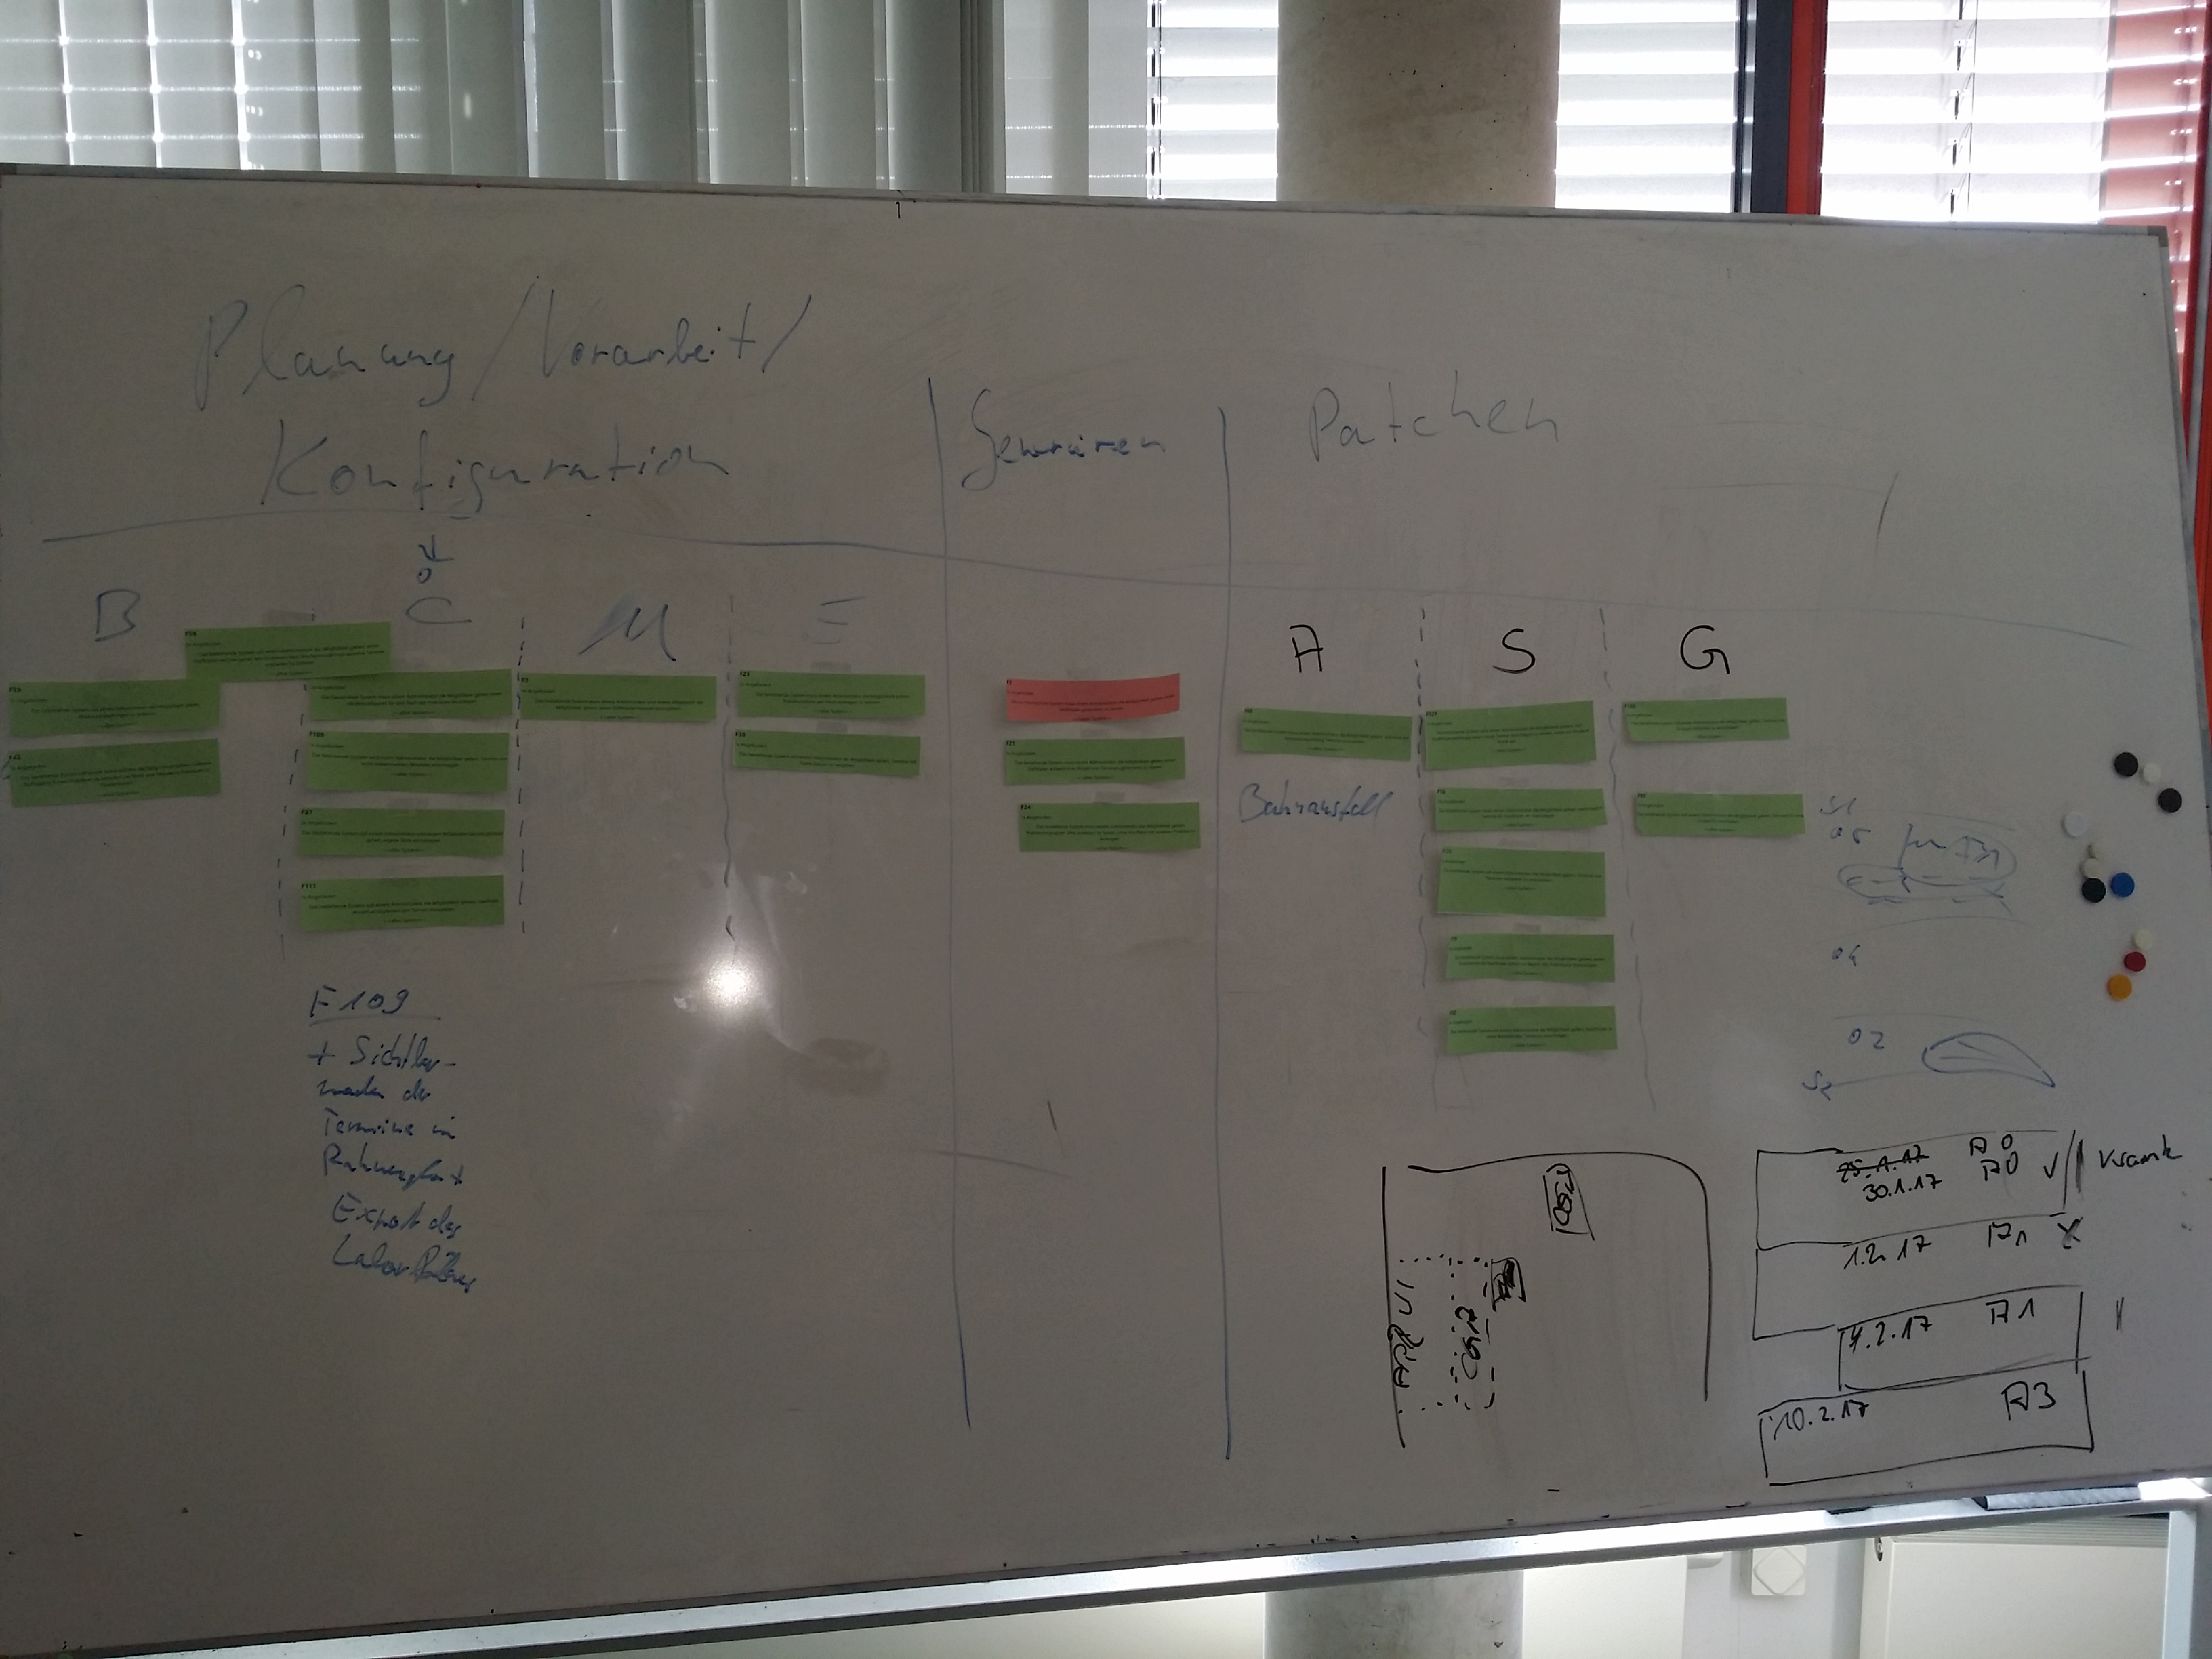
\includegraphics[width=\textwidth]{images/zweitegruppen.pdf}
\centering 
\captionabove[Gruppeneinteilung dritter \& vierter Ebene]{Gruppeneinteilung dritter \& vierter Ebene\footnotemark} 
\end{figure}
\footnotetext{Ein Bild von der Gruppeneinteilung auf dritter \& vierter Ebene an einem Whiteboard} 

Es wurde zwischen drei Ablaufphasen unterschieden, welche anschließend in weitere Teilgruppen aufgeteilt wurden.

\begin{enumerate}
\item Planung/Vorarbeit/Konfiguration
\begin{enumerate}
\item B => Blockpraktika
\item C => aktuelles Schema
\item M => manuelle Eingabe
\item F => flexible Eingaben
\end{enumerate}
\item Generieren
\item Patchen
\begin{enumerate}
\item A => betrifft alle
\item M => betrifft Studenten
\item G => betrifft Gruppen
\end{enumerate}
\end{enumerate}

Nach dieser Gruppierung sind die Anforderungen so sortiert, dass man die einzelnen Gruppen als Arbeitsschritte abarbeiten kann. Auch wurden im Laufe dieses Verfahrens neue Anforderungen aufgedeckt, die entweder aus der Sicht der Entwickler notwendig waren oder andere Anforderungen detaillieren. \\[1em]

Dieses Vorgehen wiederholt sich für alle Gruppen auf zweiter Ebene, sobald die Entwicklung des \ac{LWM}s so fortgeschritten ist, dass die nächsten Anforderungen implementiert werden können. 

\subsection{Priorisierung}
\label{subsec:priorisierung}

Die Priorisierung der Anforderungen ist notwendig, um erkennen zu können, wie wichtig eine Anforderung für die Zufriedenheit \textbf{aller} Stakeholder ist. Zudem wird diese Priorität nach der Aufwandsschätzung dazu genutzt, über die Umsetzungsreihenfolge der Anforderungen zu entscheiden.\\

Eine erste Priorisierung wurde nach der Gruppierung auf zweiter Ebene durchgeführt und wurde in Prozent angegeben. Dabei ist diese Zahl wie folgt zu interpretieren:
\begin{description}
\item $100\% \rightarrow$ \textbf{Alle} Stakeholder haben diese Anforderung als \textbf{Basisfaktor} bestimmt
\item $0\% \rightarrow$ \textbf{Kein} Stakeholder hat diese Anforderung erhoben
\end{description}

Für die Berechnung dieses Wertes wurde den einzelnen Kano-Faktoren und der Stimme eines Stakeholders (Vote) ein Wert und ein Variablen-Name zugewiesen:

\begin{description}
\item $ bap \rightarrow$ Basis-Faktor $\rightarrow$ 9
\item $ lp \rightarrow$ Leistungs-Faktor $\rightarrow$ 6
\item $ bep \rightarrow$ Begeisterungs-Faktor $\rightarrow$ 3
\item $ vp \rightarrow$ Vote $\rightarrow$ 1
\end{description}

Des Weiteren werden folgende Parameter benötigt:
\begin{description}
\item $ v \rightarrow$ die Votes der Anforderung
\item $ m \rightarrow$ die maximalen Votes die für eine Anforderung abgegeben wurden
\item $ p \rightarrow$ die Priorität in \%
\end{description}

Die Formel sieht dann wie folgt aus:
$$ p = \frac{v * vp + <bap|lp|bep>}{m*vp + bap}$$

Nachdem die Aufwandsschätzung abgeschlossen war, konnte mit dem dort geschätzten Wert und der Priorität deutlich gemacht werden, wie die Anforderung im Laufe der Entwicklung zu interpretieren ist.\\

Um die weitere Berechnung verstehen zu können, ist es wichtig zu wissen, dass die Komplexität einer Anforderung in Story-Points geschätzt wurde. Hierbei bedeuten 10 Story-Points, dass die Anforderung einen hohen Implementierungsaufwand mit sich bringt und 1 Story-Point, dass die Implementierung dieser am wenigsten komplex ist.\\

Das Prinzip dieser Interpretation wird mit der Abbildung \ref{fig:erklärung} deutlich.


\begin{figure}[!htb]
		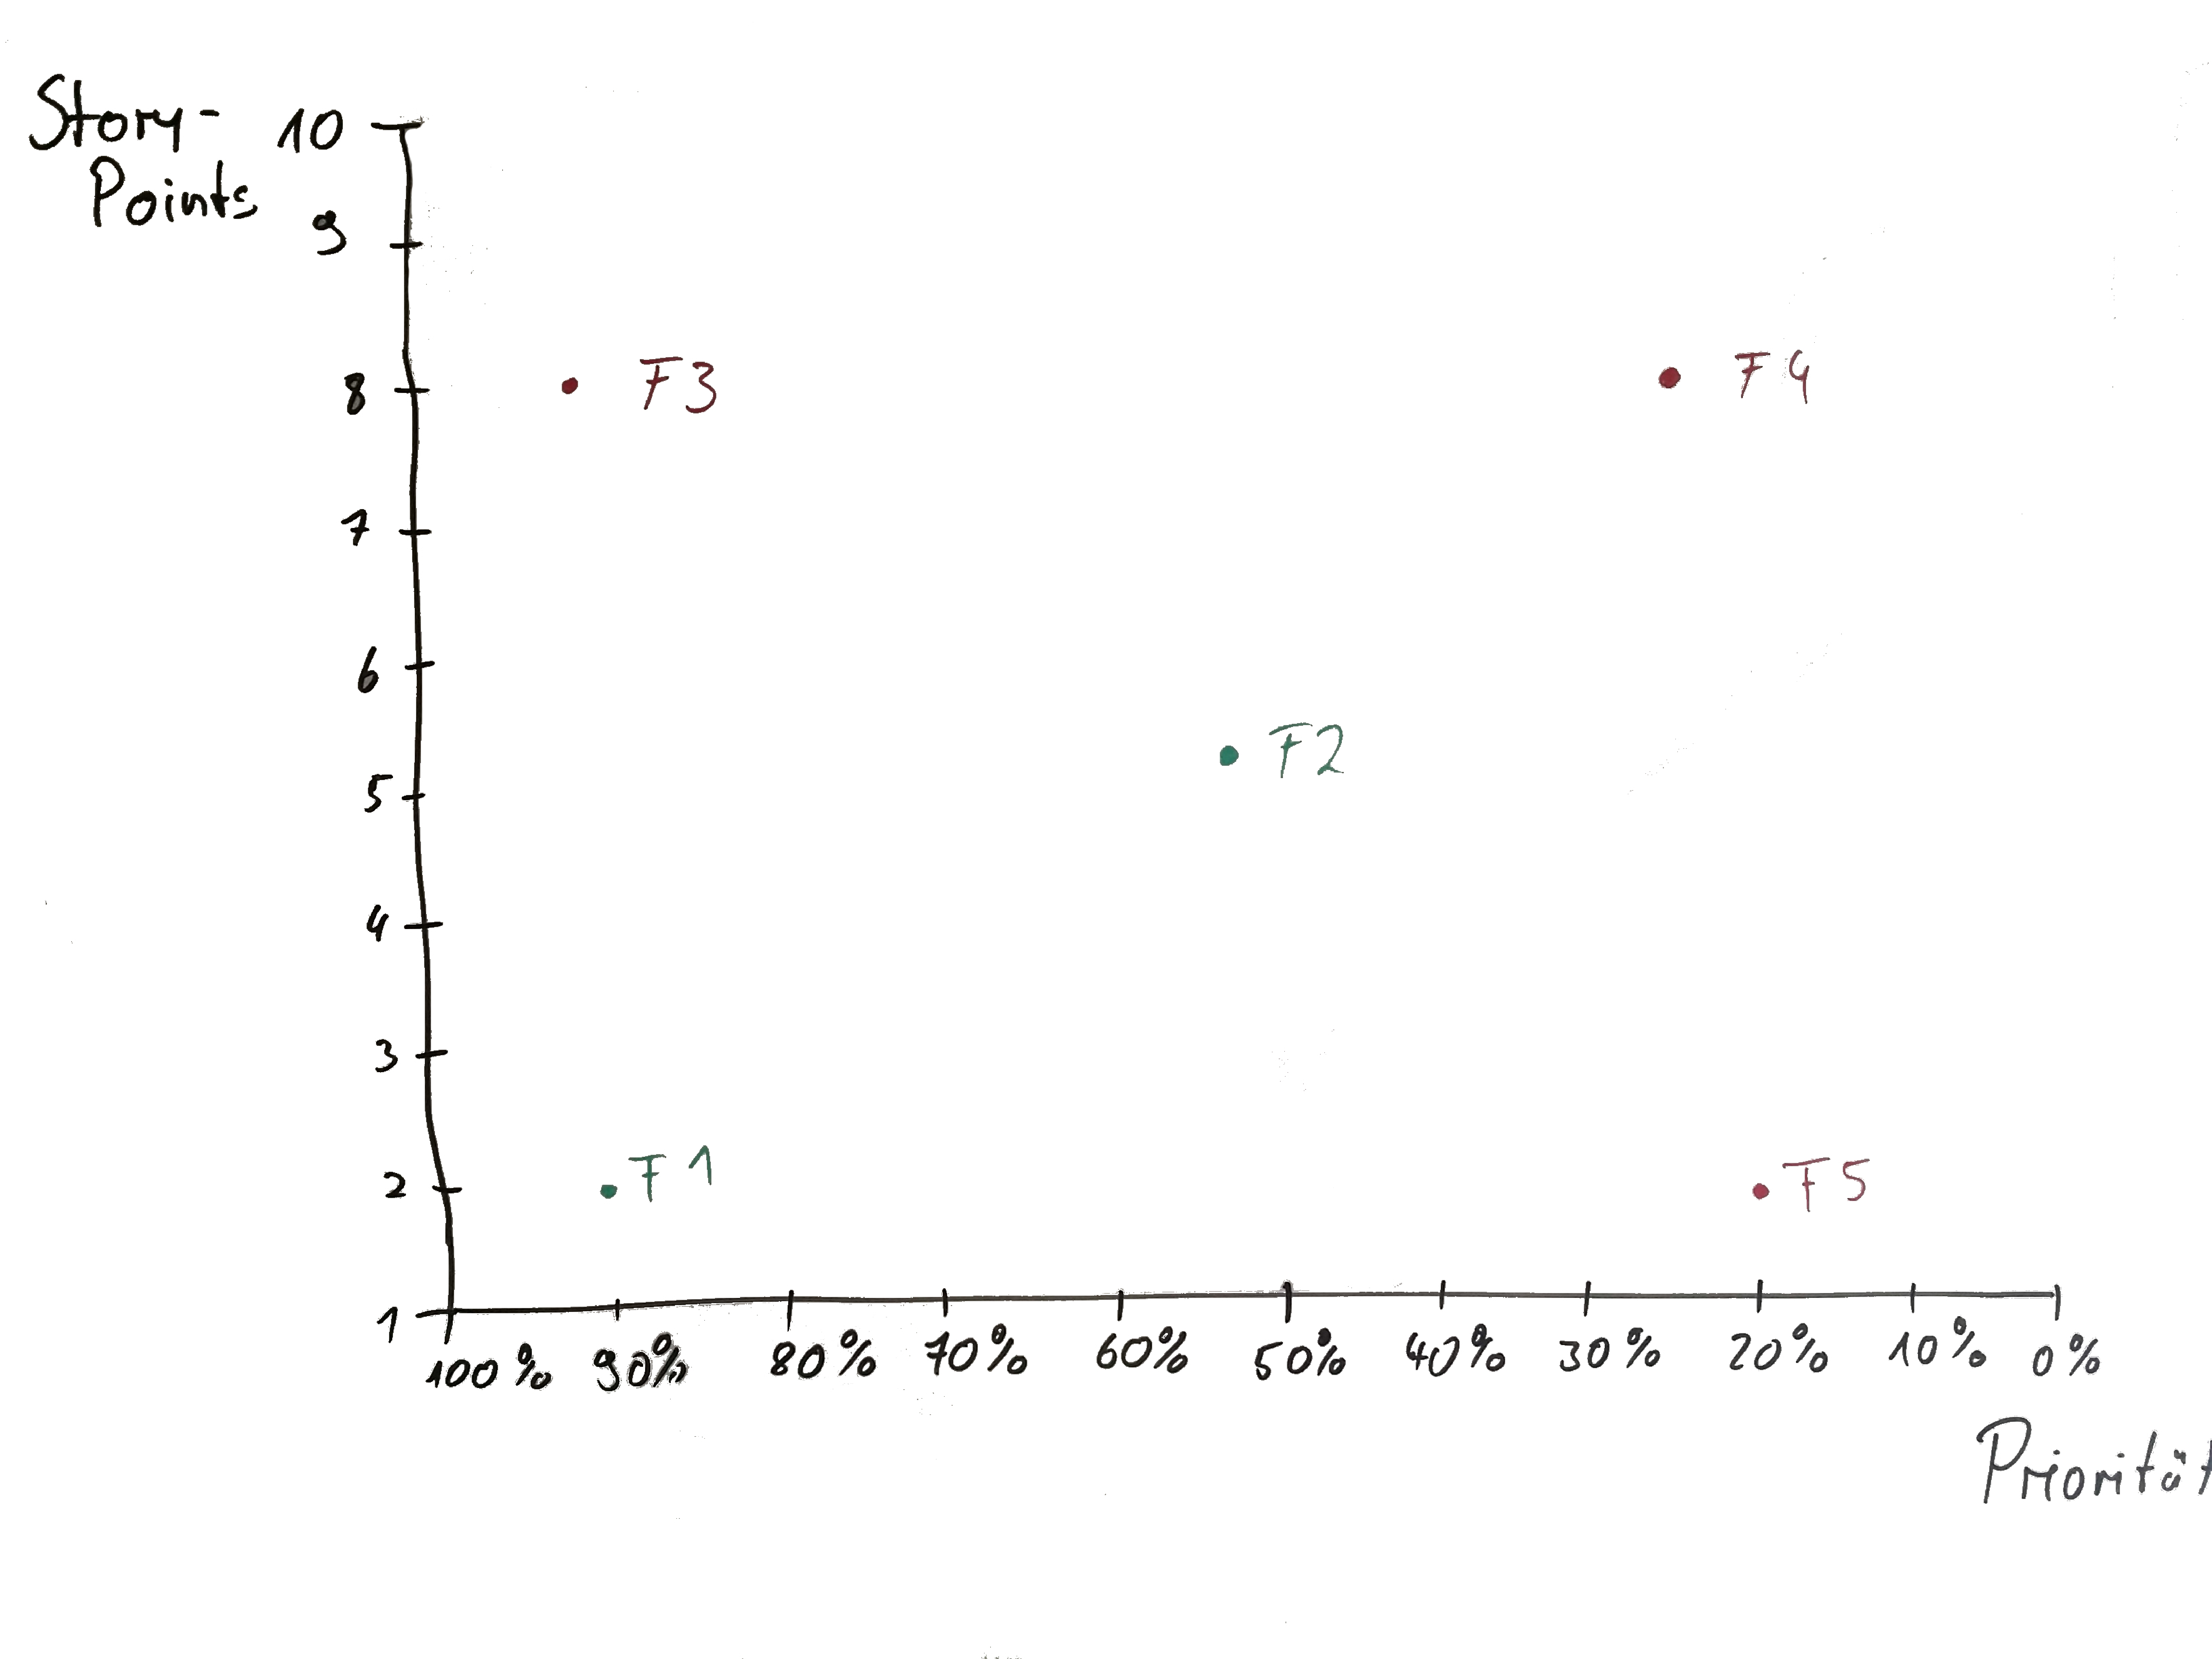
\includegraphics[width=\textwidth]{images/ergebnis.pdf}
\centering 
\captionabove[Erklärung der Anforderungsauswertung]{Erklärung der Anforderungsauswertung\footnotemark} 
  \label{fig:erklärung}
\end{figure}
\footnotetext{Erklärung der Anforderungsauswertung anhand eines Beispiels} 

Auf Abbildung \ref{fig:erklärung} ist zu erkennen, dass die Anforderung \textit{F3} zwar einen hohen Implementierungsaufwand bedeutet, diese allerdings eine Stakeholder-Priorität von 90\% aufweist. Dagegen hat \textit{F5} nur eine Priorität von 20\%, jedoch ist diese auch wesentlich einfacher erfüllbar. Diese beiden Anforderungen haben also in erster Linie keine hohe Priorität bei der Entwicklung. \textit{F4} weist von den abgebildeten Beispielen die schlechteste Bewertung auf. Diese ist, wenn überhaupt, erst ganz am Ende zu betrachten, wenn alle anderen Anforderungen erfüllt wurden. \textit{F1} hingegen ist sofort umzusetzen, da diese nicht nur von den meisten Stakeholdern als wichtig angesehen wurde, sondern auch relativ einfach zu implementieren ist. \\[1em]

Durch die Abarbeitung in dieser Reihenfolge können die wichtigsten Wünsche der Stakeholder am schnellsten erfüllt werden, deshalb wurde für die Anforderungen bei diesem Projekt auch ein solcher Wert berechnet. Wie die Berechnung als Formel aussieht, wird nachfolgend gezeigt. Doch vorher muss auch für diese Formel die Definition einiger Variablen geklärt werden:

\begin{description}
\item $ sp \rightarrow$ die Story-Points die der Anforderung bei der Aufwandsschätzung zugewiesen wurde
\item $ p \rightarrow$ die Priorität der Anforderung in \%
\item $ r \rightarrow$ das Ergebnis der Berechnungen. (Da für diese Variable kein passender Name gefunden werden konnte, wird diese ab jetzt auch weiterhin Ergebnis genannt)
\end{description}

Nun ist es es ohne Probleme möglich, die Formel zu verstehen:
$$r = 100-\sqrt{(sp-1)^{2}+(100-p)^{2}}$$
Der Kern dieser Formel ist der Satz des Pythagoras:
$$c^{2} = a^{2}+ b^{2} \rightarrow c = \sqrt{a^{2}+ b^{2}}$$
Hierbei ist $c$ unser Ergebnis $r$, $a$ sind die Story-Points $- 1$. \\

\textbf{Doch warum Story-Points $- 1$?}\\
Wie in Kapitel \ref{subsec:validation} (\nameref{subsec:validation}) beschrieben wurde, konnte im Vorfeld entschieden werden, ob eine Anforderung als \textit{"Erledigt"}, \textit{"Valide"} oder \textit{"Verworfen"} anzusehen ist. Bei der weiteren Auswertung sind erledigte oder verworfene Anforderungen kaum noch von Interesse, deshalb werden diese in der Berechnung nicht beachtet. Das hat zur Folge, dass eine Anforderung, welche in diese Berechnung mit einfließt, einen Mindestaufwand von einem Story-Point haben muss. Schließlich gibt es keine noch nicht implementierte Anforderung, deren Realisierung keinen Aufwand mit sich zieht.\\

Mit der Rechnung "Story-Points $- 1$" wurde also eine Normalisierung durchgeführt, um mit einem Story-Point und 100\% Priorität auch ein Ergebnis von 100\% zu erzielen, denn das ist das Beste was eine Anforderung haben kann. \\

Schließlich ist noch das $b$ zu betrachten. Dieses wird durch $100-p$ ersetzt, wobei $p$ die Priorität der Anforderung ist, welche ohne Berücksichtigung der Komplexität errechnet wurde. Warum diese Priorität von 100 abgezogen wird, erkennt man in Abbildung \ref{fig:erklärung100-p}.


\begin{figure}[!htb]
\centering 
		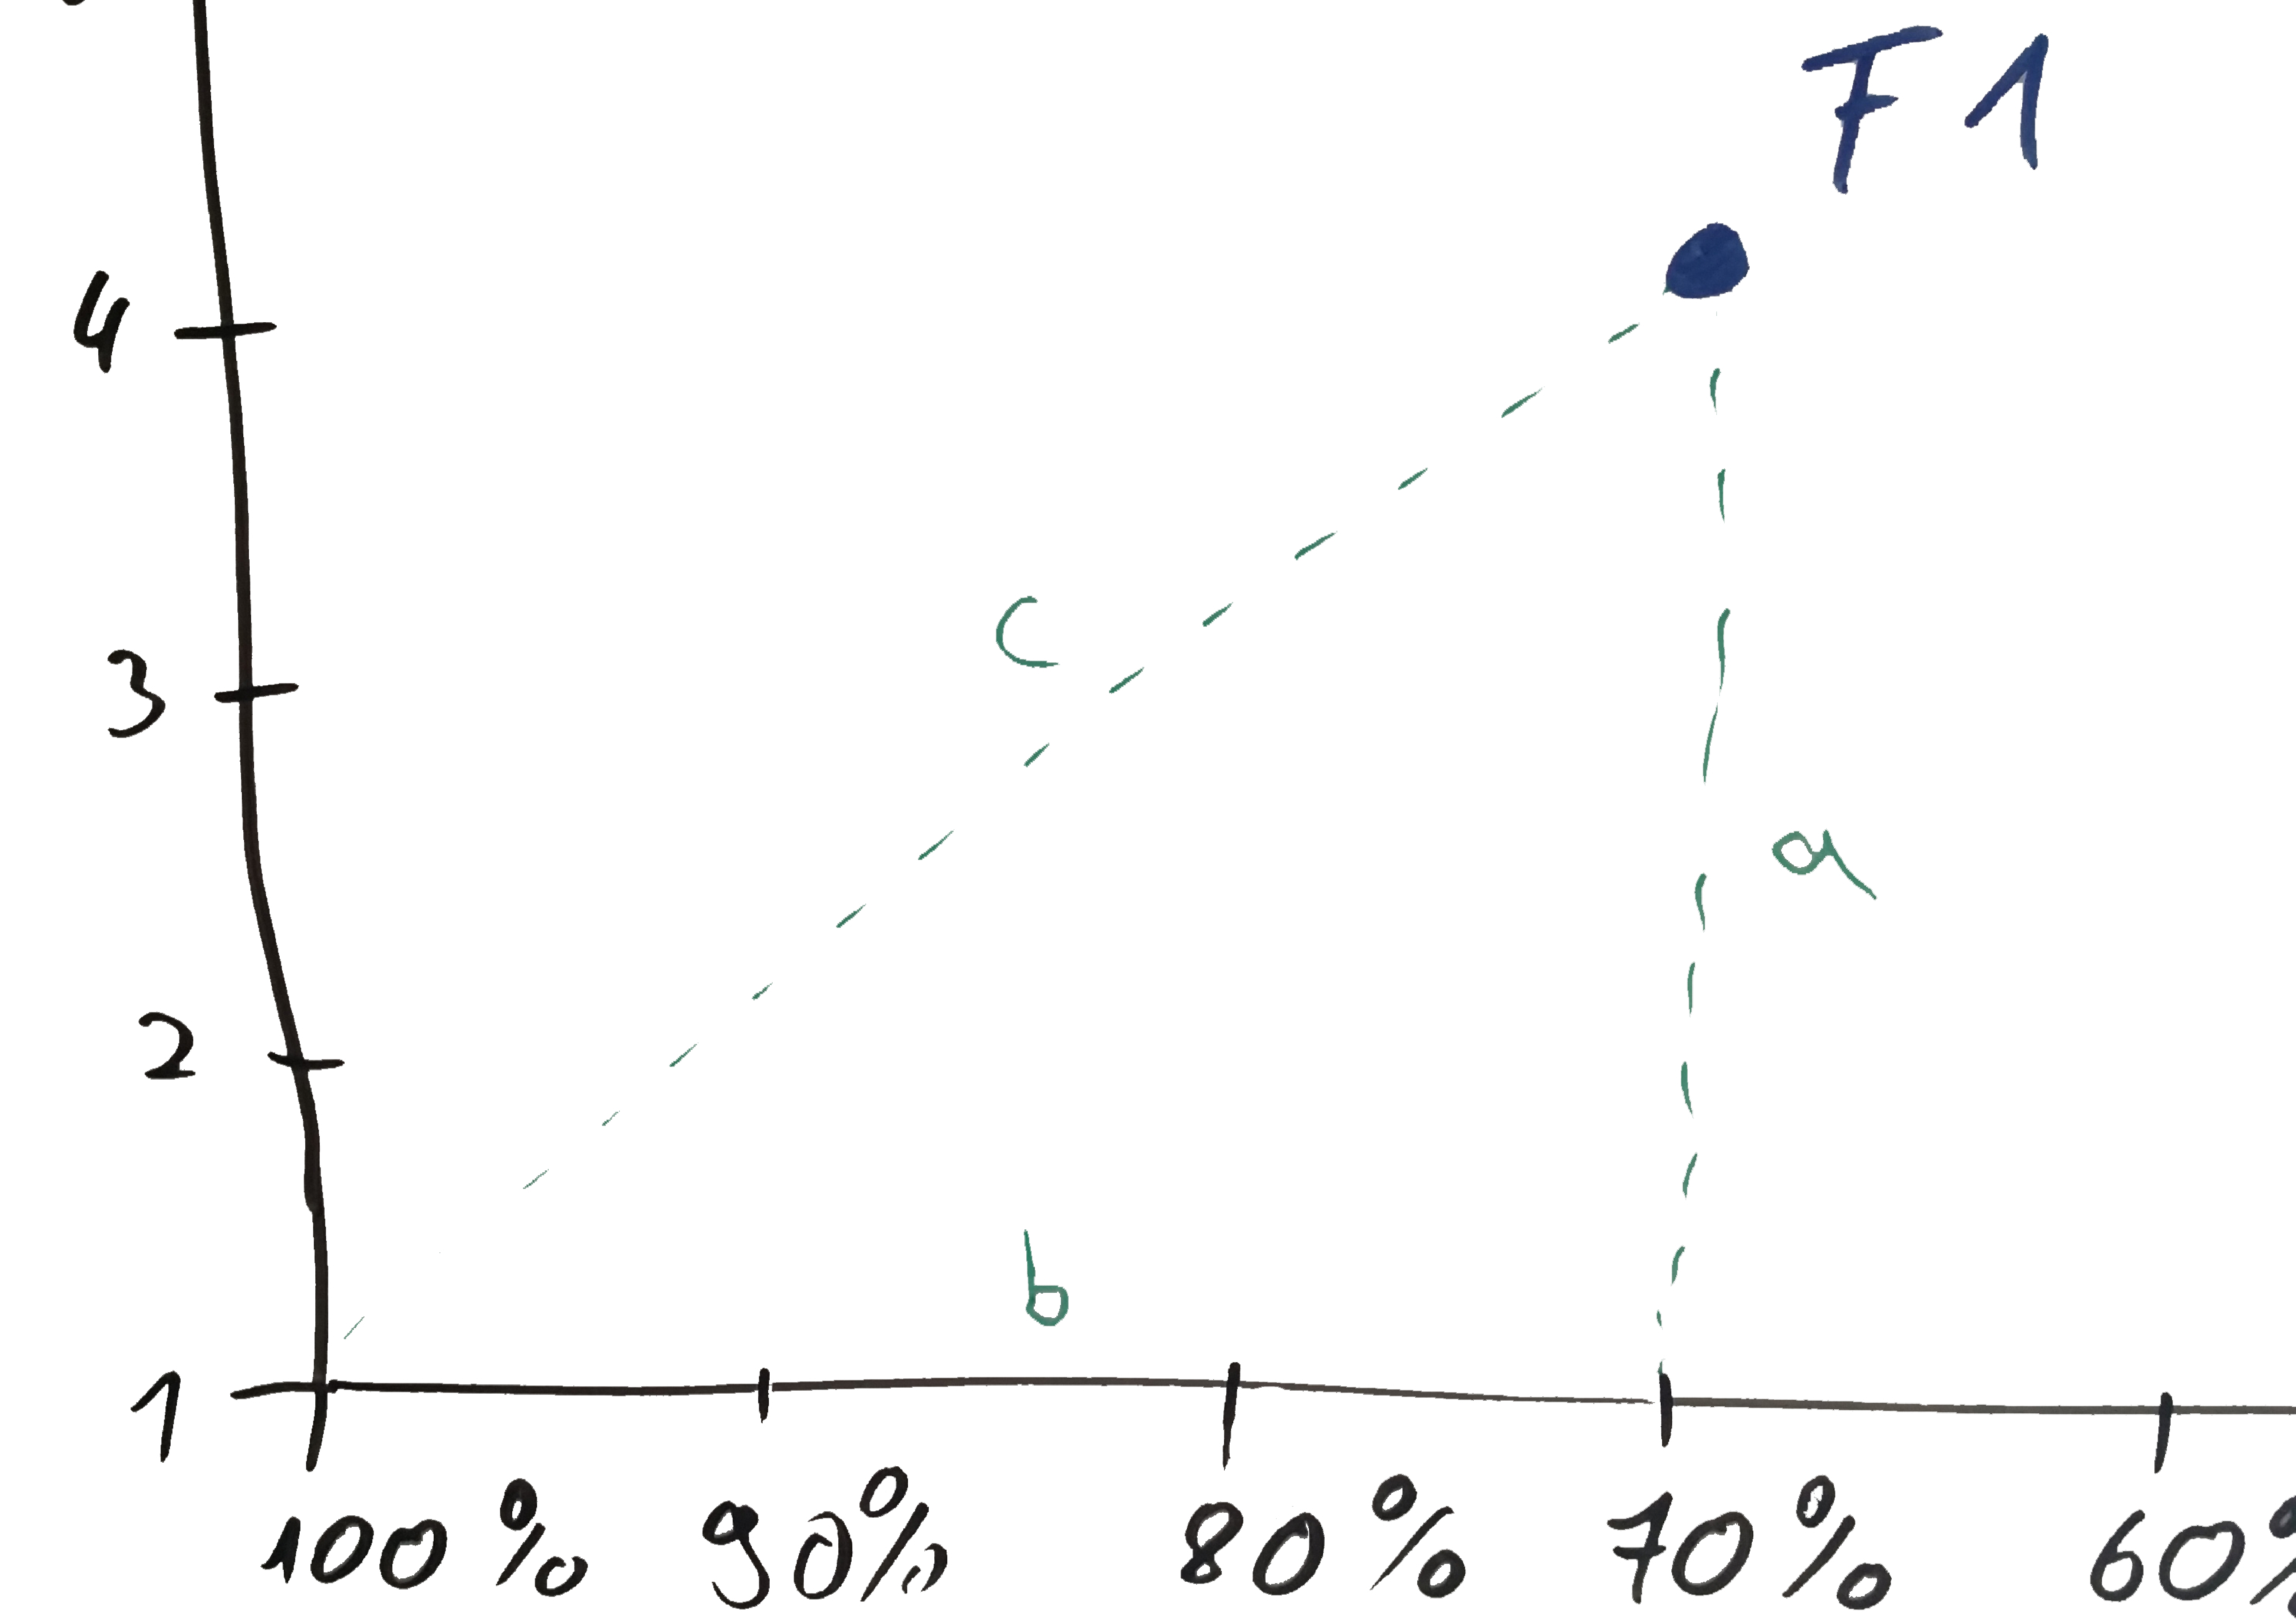
\includegraphics[width=0.5\textwidth]{images/100minusp.pdf}
\captionabove[Erklärung zur Rechnung 100 - p]{Erklärung zur Rechnung 100 - p\footnotemark} 
  \label{fig:erklärung100-p}
\end{figure}
\footnotetext{Eine Bild zur Erklärung für die Rechnung 100 - p bei der Priorisierung} 

Die y-Achse stellt die Skala der Priorität dar. Da laut der durchgeführten Rechnung $c$, also die Länge des Ortsvektor, die Bewertung der Anforderung darstellt, ist zu beachten, dass die y-Achse am Koordinatenursprung mit $100\%$ beginnt. Somit stellt eine Priorität von $70\%$ für $b$ nicht den Wert 70 dar, sondern $100-70$ also $30$.\\[1em]

Nachdem diese Berechnungen und somit die Bewertung der Anforderungen durchgeführt wurde, ist es dem Entwickler-Team möglich, die Anforderungen mit der richtigen Priorität zu implementieren.


\subsection{Aufwandsschätzung}
\label{subsec:aufwandsschätzung}

Bei der Aufwandsschätzung der ermittelten Anforderungen wurde sich aufgrund der agilen Entwicklung des \ac{LWM}s bewusst gegen die Anwendung der \ac{FPA} oder anderen klassischen Schätzmethoden entschieden. Statt dessen wurde an dieser Stelle von \ac{SP} Gebrauch gemacht. Der Grund dafür liegt neben dem hohen Aufwand einer Function-Point-Analyse in Erfahrungsberichten, die ebenfalls dazu raten.

\begin{quote}
\glqq Die Erfahrung (nicht nur der agilen Projektwelt) hat aber gezeigt, dass das vergleichende Schätzen in abstrakten Schätzmaßen zu deutlich schnelleren und besseren Ergebnissen führt.\grqq    \citep{AGIL1}
\end{quote}

Um eine Schätzung mit \acl{SP} durchführen zu können, werden die Anforderungen in eine \ac{US} aufgeteilt. Diese Storys bekommen anschließend Story-Points zugewiesen. In diesem Fall wurde ein Intervall von 1 - 10 festgelegt, wobei 1 für eine niedrige und 10 für eine sehr hohe Komplexität steht. Hierbei ist zu unterscheiden, dass, im Gegensatz zu klassischen Schätzverfahren, nicht der Aufwand sondern die Komplexität geschätzt wird. \\[1em]

Damit nun die Story-Points ordnungsgemäß zugewiesen werden konnten, wurde eine Anforderung rausgesucht, welche einen guten Mittelwert an Komplexität bedeutet. Dieser Anforderung wurden die ersten Punkte zugewiesen. Relativ zu dieser Schätzung wurde anschließend auch den übrigen Anforderungen ein Wert gegeben. Dieser Prozess wurde in einem Meeting mit dem Entwickler-Team vor Ort, im Zuge der detaillierteren Gruppierung, durchgeführt. Dazu haben sich die Entwickler von Frontend und Backend zu der Komplexität der jeweiligen Implementierung abgesprochen und sich auf eine Anzahl an Story-Points geeinigt. Dieses Verfahren kann man, genauso wie die Gruppierung, auch in weiteren Iterationen weiter verfeinern. Dazu werden diese \ac{US} wieder in kleinere aufgesplittet, welche wiederum \ac{SP} zugewiesen bekommen. Dieser Vorgang ist bei sehr groben \ac{US} zu empfehlen.\\[1em]

Die somit verteilten \ac{SP} konnten anschließend zur weiteren Priorisierung genutzt werden.

\chapter{Visualisierung der Ergebnisse}

Die ermittelten Anforderungen sollen, auch nach der Fertigstellung dieses Projekts, noch zur Orientierung bei der Entwicklung des \ac{LWM} dienen. Deshalb ist eine ordnungsgemäße und langfristige Speicherung der Anforderungen unumgänglich. Für die weitere Auswertung und Priorisierung ist es zudem notwendig, Berechnungen und Sortierungen mit den Anforderungen durchzuführen. \\[1em]

\section{Excel}
\begin{figure}[!htb]
		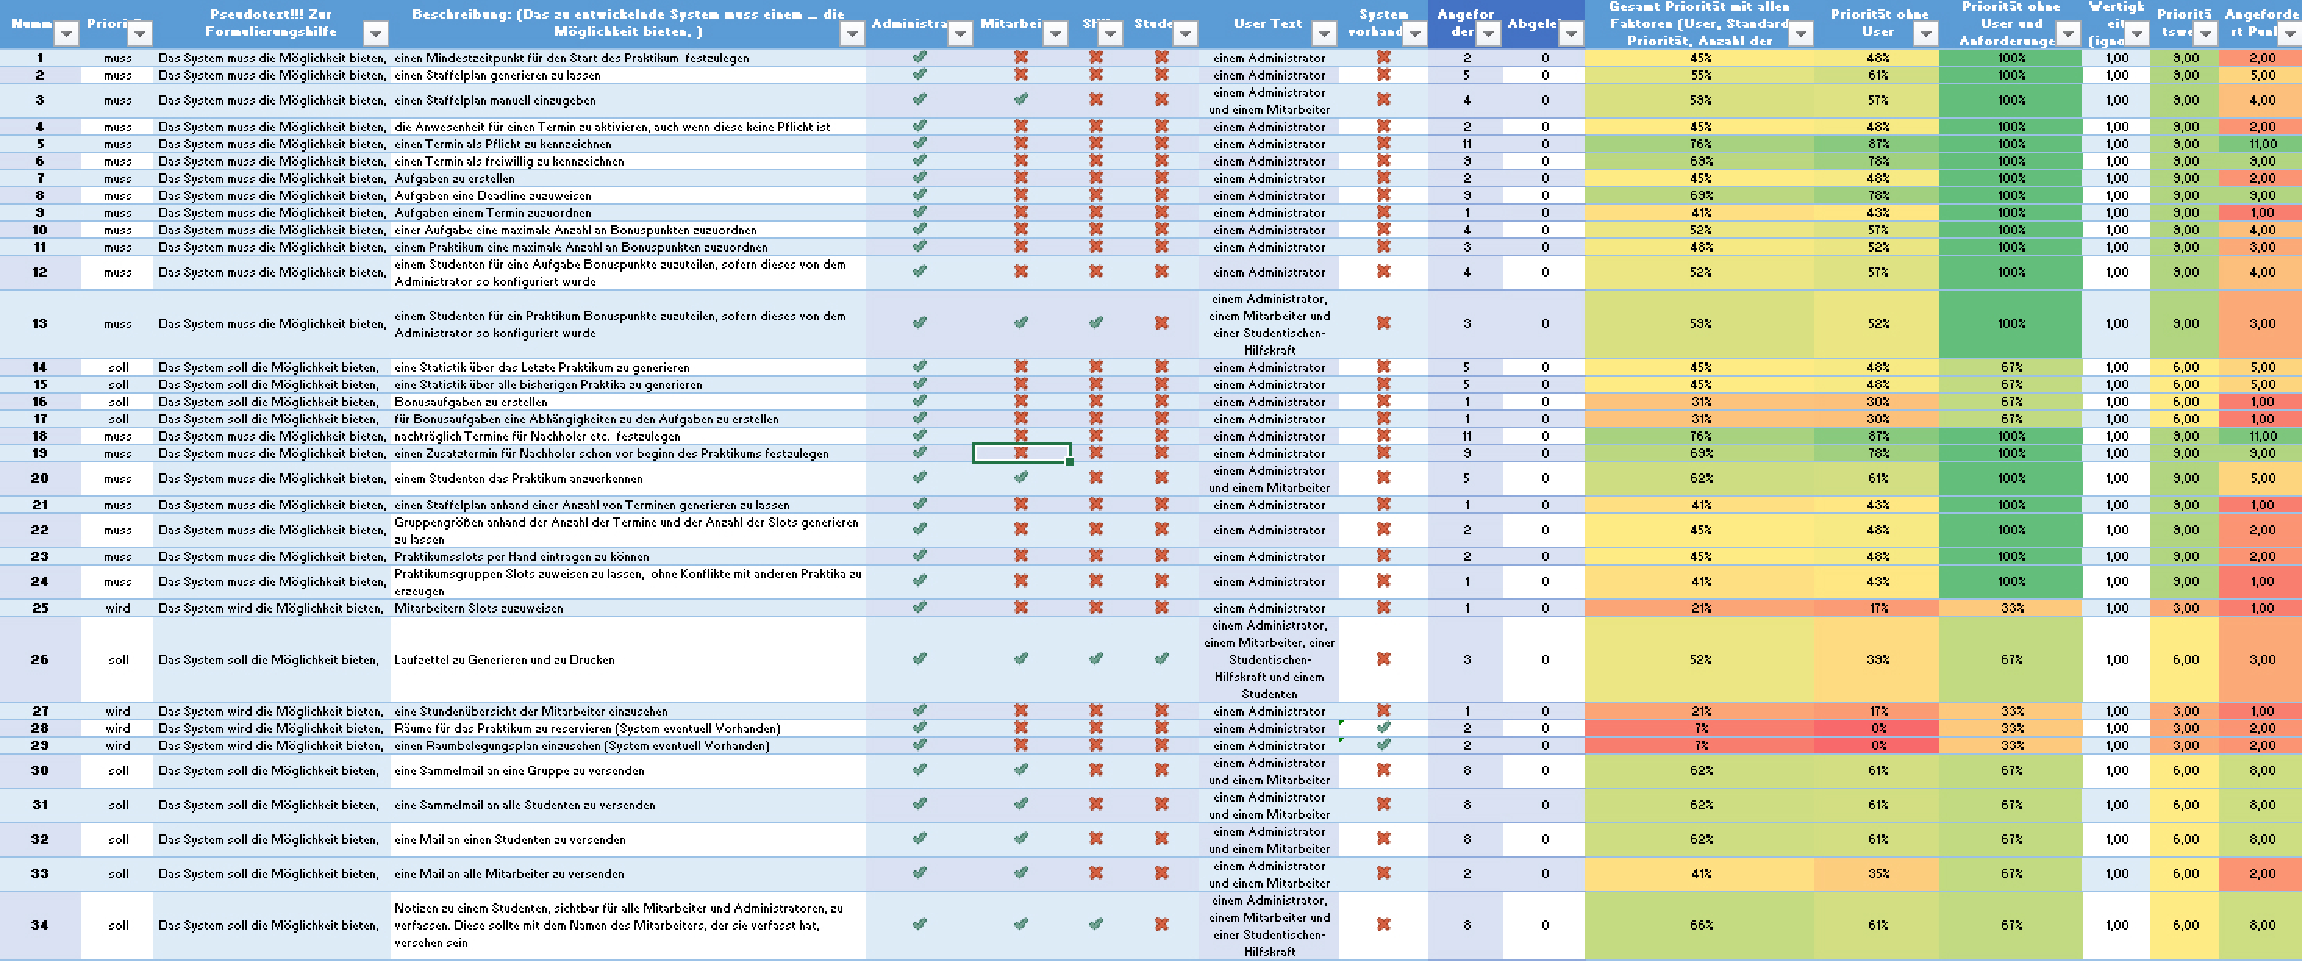
\includegraphics[width=\textwidth]{images/excel.pdf}
\centering 
\captionabove[Ausschnitt aus Excel]{Ausschnitt aus Excel\footnotemark} 
		\label{fig:excel}
\end{figure}
\footnotetext{Ein Ausschnitt aus der Dokumentation der Anforderungen in Excel} 
Der erste Ansatz war das Dokumentieren in Excel. Dort wurden (wie in Abbildung \ref{fig:excel} zu sehen) alle Anforderungen aufgenommen und erste Berechnungen der Prioritäten durchgeführt. Jedoch stellte sich im Laufe dieser Bearbeitung heraus, dass Excel nicht alle Funktionalitäten, die benötigt wurden, zufriedenstellend bereitgestellt. Zudem erfolgt die Speicherung der Daten in einer lokalen Datei, was deren aktive Nutzung von mehreren Beteiligten erschwert. Also wurde die Entscheidung getroffen ein Programm zum Verwalten der Daten zu entwickeln, damit dort alle notwendigen Funktionen nach belieben implementiert werden können.


\section{Website}

Eine einfache und effektive Lösung der Datenhaltung und -verarbeitung bot die Kombination einer Angular2-Webseite und einer MySQL-Datenbank. Durch vorherige Projekte bestand derzeit schon der Zugang zu einem Server und einer Datenbank, was diese Entscheidung stützte. Zudem ist die Erstellung einer Angular2-Webseite mit weniger Aufwand verbunden als ein Java-Programm, welches die andere Alternative gewesen wäre.\\

Durch diese Website bestand die Möglichkeit, auch ohne eine persönliche Zusammenkunft, mit dem Entwickler-Team einige Absprachen und Anpassungen durchzuführen. So konnten nicht nur dynamisch neue Anforderungen über ein perfekt dafür zurecht geschnittenes Interface hinzugefügt und mit den nötigen Informationen bestückt werden (Abbildung \ref{fig:erstellen}), sondern auch die Editierung dieser konnte, in die davon abhängigen Berechnungen, sofort mit einbezogen werden.\\

\begin{figure}[!htb]
		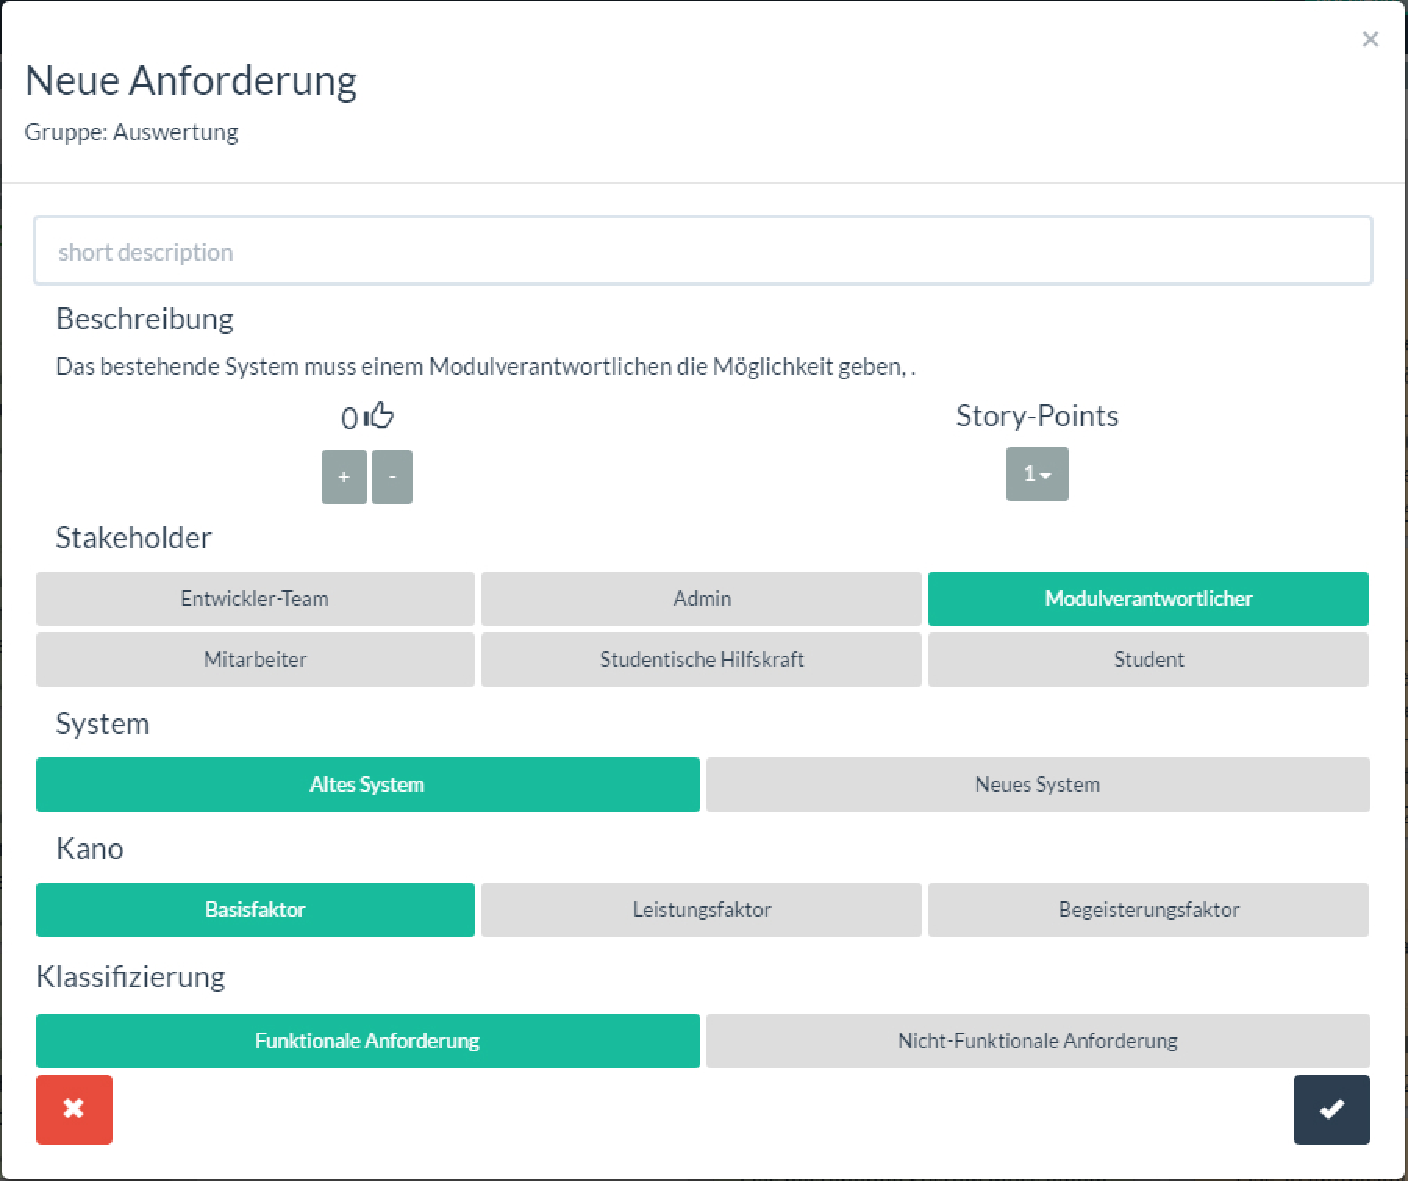
\includegraphics[width=.5\textwidth]{images/erstellen.pdf}
\centering 
\captionabove[Erstellen einer Anforderung]{Erstellen einer Anforderung\footnotemark} 
		\label{fig:erstellen}
\end{figure}
\footnotetext{Erstellen einer Anforderung mit einem eigens dafür konzipierten Interface} 


\subsection{Gruppen}
Ein weiterer Vorteil dieser Entscheidung war das einfache Gruppieren der Anforderungen. Um eine Anforderung einzufügen, wird diese direkt der jeweiligen Gruppe über den "Plus-Button" hinzugefügt. Sofern eine bestehende Anforderung in eine neue Gruppe geschoben werden soll, kann dies mittels "Drag and Drop" realisiert werden. Auch bei diesem Vorgang werden alle Folgeberechnungen angepasst. Auch die Übersicht dieser Gruppen ist in dieser App wesentlich besser als sie in Excel gewesen wäre (siehe Abbildung \ref{fig:gruppen}).

\begin{figure}[!htb]
		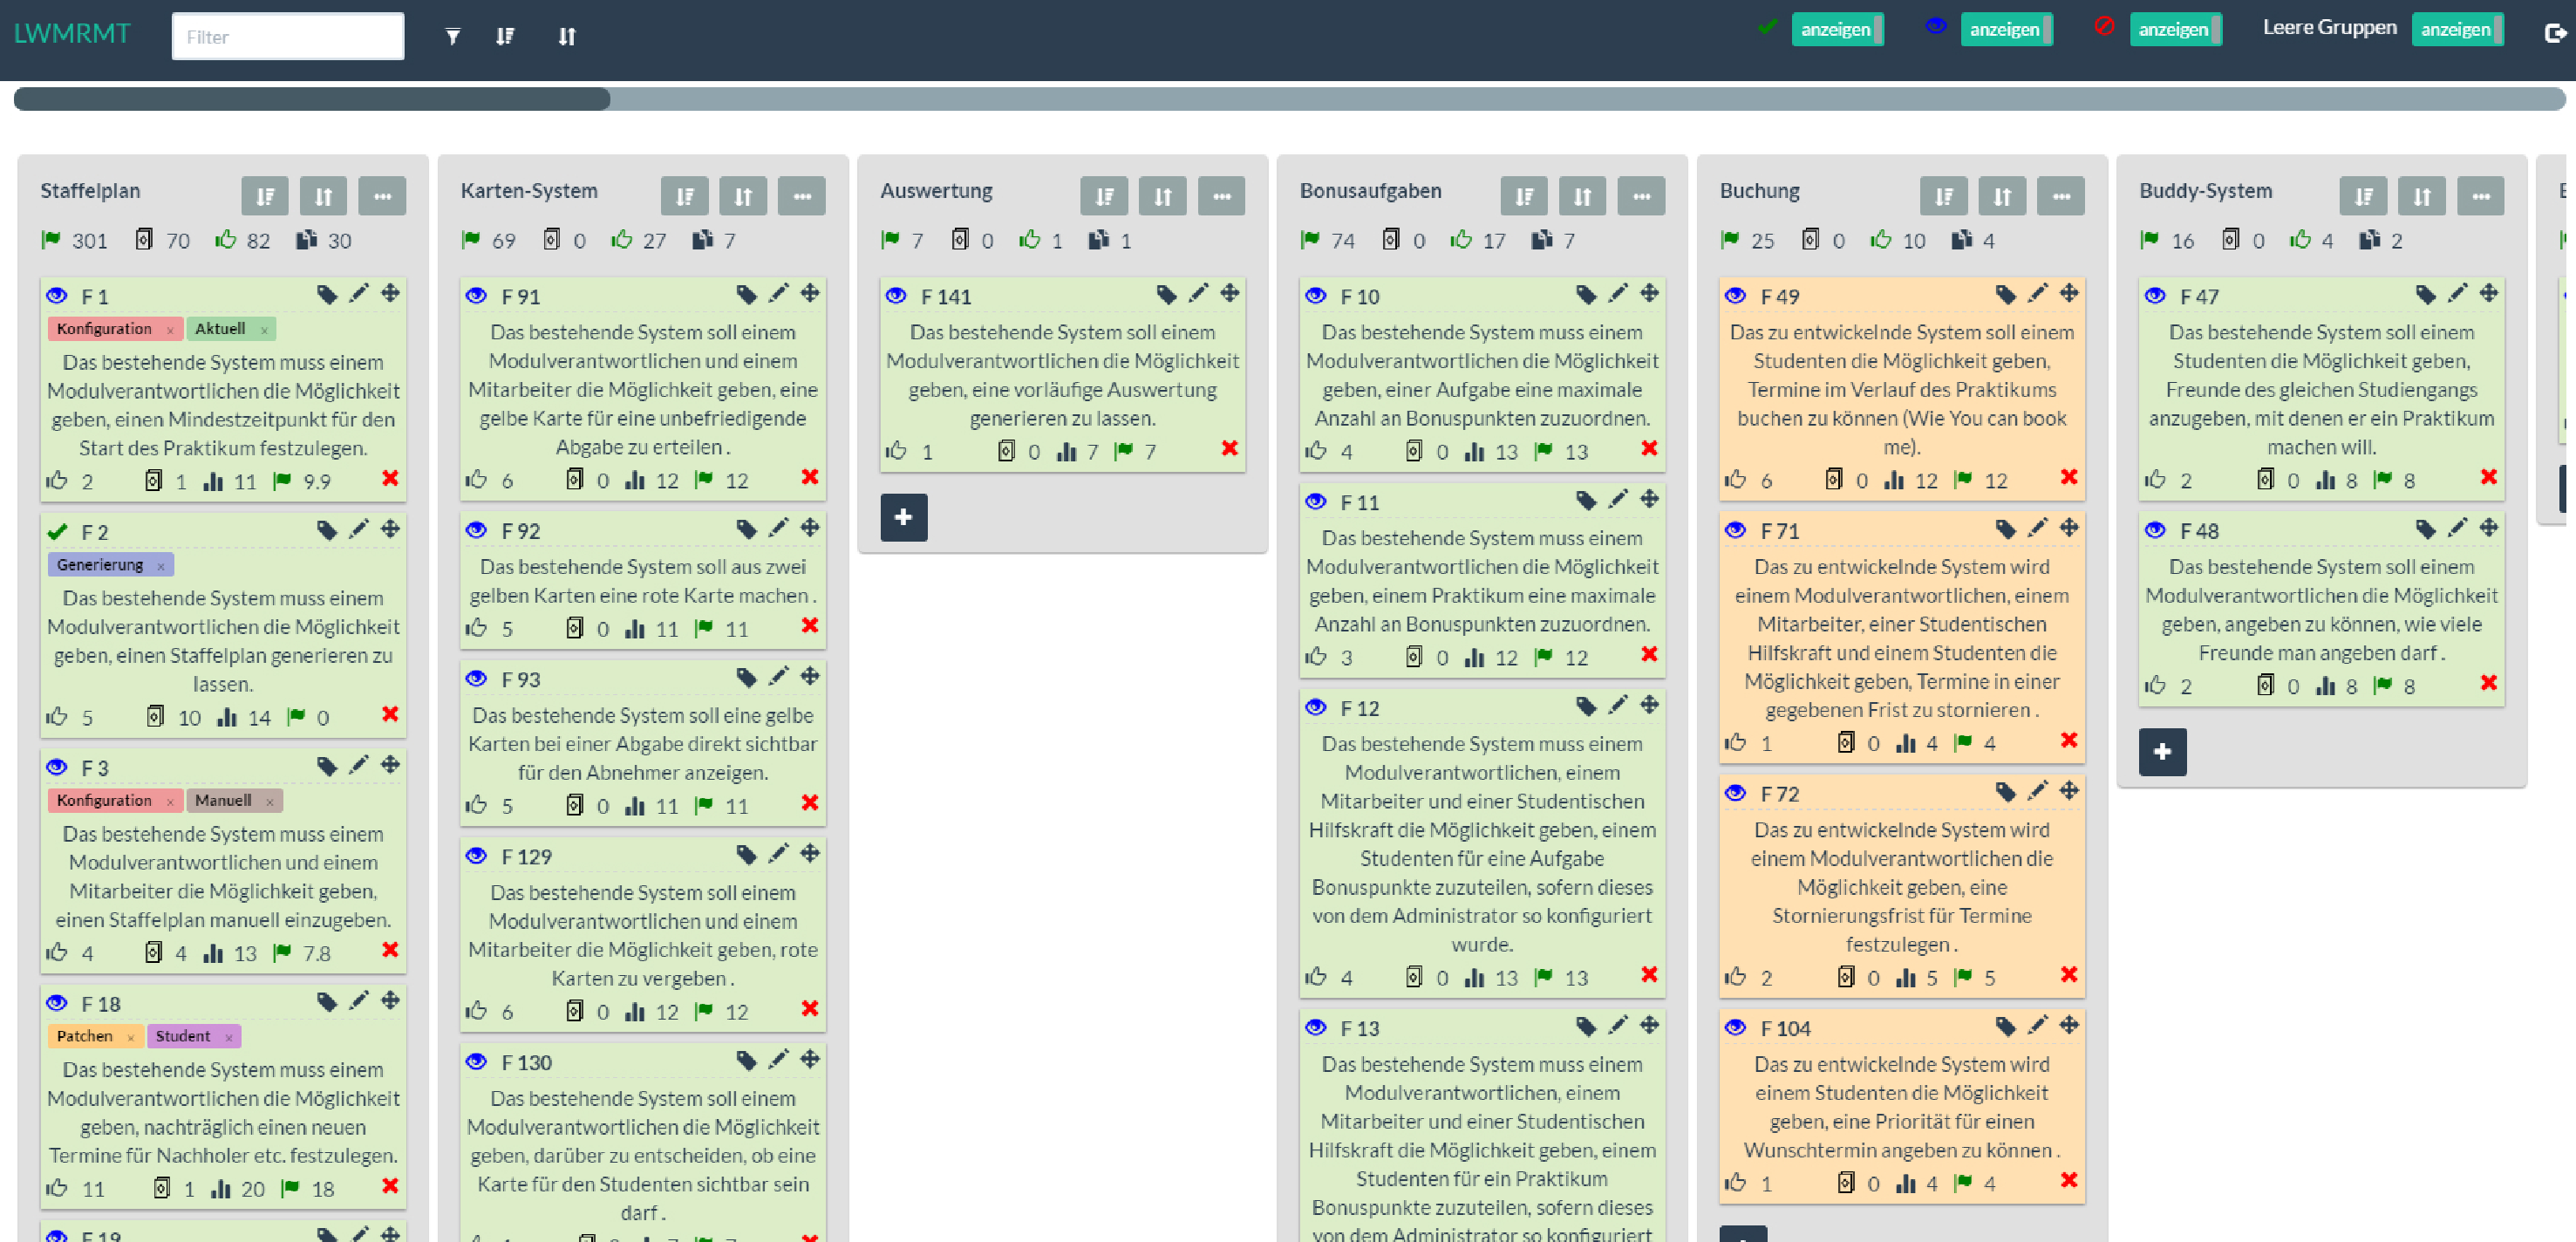
\includegraphics[width=\textwidth]{images/webseite.pdf}
\centering 
\captionabove[Ausschnitt der Webseite]{Ausschnitt der Webseite\footnotemark} 
\label{fig:gruppen}
\end{figure}
\footnotetext{Ein Ausschnitt aus der Dokumentation der Anforderungen mit der Webseite} 


\subsection{Labels}
Das Programm bietet zudem ein Interface, mit dem man Labels für eine Gruppe erstellen kann (Abbildung \ref{fig:labelerstellen}).

\begin{figure}[!htb]
		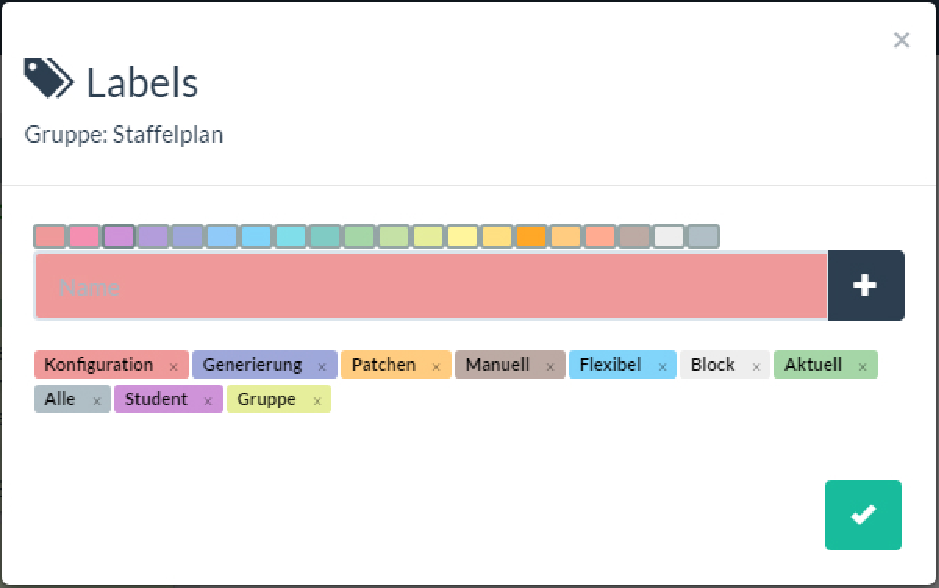
\includegraphics[width=.5\textwidth]{images/labelserstellen.pdf}
\centering 
\captionabove[Erstellen eines Labels]{Erstellen eines Labels\footnotemark} 
\label{fig:labelerstellen}
\end{figure}
\footnotetext{Das Erstellen eines Labels in einer Gruppe über das User-Interface}

Diese können anschließend den Anforderungen dieser Gruppe zugeordnet werden (Abbildung \ref{fig:labelzuordnen}). 

\begin{figure}[!htb]
		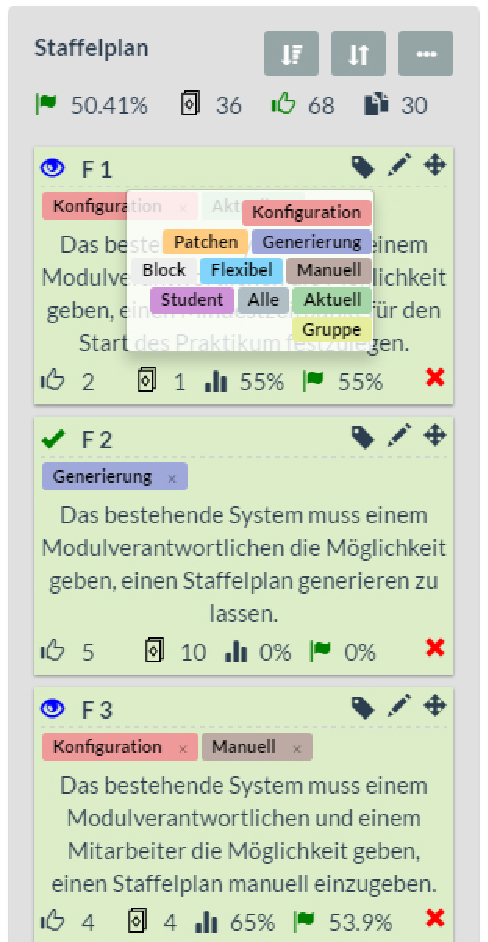
\includegraphics[width=.25\textwidth]{images/labelzuordnen.pdf}
\centering 
\captionabove[Zuordnen eines Labels]{Zuordnen eines Labels\footnotemark} 
\label{fig:labelzuordnen}
\end{figure}
\footnotetext{Zuordnen eines Labels zu einer Anforderung mit dem User-Interface} 

\subsection{Informationen}
Die Anforderungen selbst bieten alle nötigen Informationen auf einem Blick, wie in Abbildung \ref{fig:anforderung} zu erkennen ist.

\begin{figure}[!htb]
		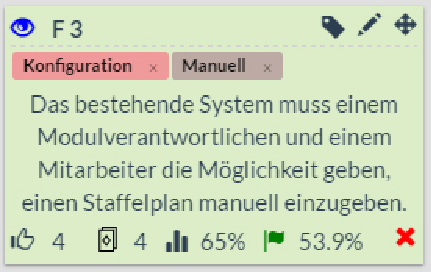
\includegraphics[width=.5\textwidth]{images/anforderung.pdf}
\centering 
\captionabove[Eine Anforderung im User-Interface]{Eine Anforderung im User-Interface\footnotemark} 
\label{fig:anforderung}
\end{figure}
\footnotetext{Die Detail-Ansicht einer Anforderung im User-Interface}

Hier sind nicht nur die zugewiesenen Labels zu erkennen, sondern diese Karte zeigt alle Informationen über diese Anforderung. 

\begin{figure}[!htb]
		
\includegraphics[width=0.05\textwidth]{images/thumbs.pdf}
	\textit{Die Anzahl der Votes}
\end{figure}
\vspace{-15pt}
\begin{figure}[!htb]
		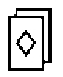
\includegraphics[width=0.05\textwidth]{images/cards.pdf}
	\textit{Die Anzahl der Story-Points}
\end{figure}
\vspace{-15pt}
\begin{figure}[!htb]
		
\includegraphics[width=0.05\textwidth]{images/stats.pdf}
	\textit{Die Priorität in \%}
\end{figure}
\vspace{-15pt}
\begin{figure}[!htb]
		
\includegraphics[width=0.05\textwidth]{images/flag.pdf}
	\textit{Das Ergebnis in \%}
\end{figure}
\vspace{-15pt}
\begin{figure}[!htb]
		
\includegraphics[width=0.05\textwidth]{images/eye.pdf}
	\textit{Der Status der Anforderung, in diesem Fall "Valide"}
\end{figure}
\vspace{-15pt}
\begin{figure}[!htb]
		
\includegraphics[width=0.05\textwidth]{images/ok.pdf}
	\textit{Der Status der Anforderung, wenn sie "Erledigt" ist}
\end{figure}
\vspace{-15pt}
\begin{figure}[!htb]
		
\includegraphics[width=0.05\textwidth]{images/ban.pdf}
	\textit{Der Status der Anforderung, wenn sie "Verworfen" ist}
\end{figure}

\pagebreak
Auch eine Gruppe hat alle Informationen direkt ersichtlich, die dort verwendeten Zeichen haben die gleiche Bedeutung wie bei einer Anforderung, mit dem Unterschied, dass diese Daten sich aus den Anforderungen der Gruppe zusammensetzen (Abbildung \ref{fig:gruppeninfo}).

\begin{figure}[!htb]
		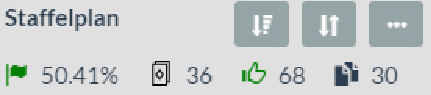
\includegraphics[width=.5\textwidth]{images/groupinfo.pdf}
\centering 
\captionabove[Gruppeninformationen]{Gruppeninformationen\footnotemark} 
\label{fig:gruppeninfo}
\end{figure}
\footnotetext{Die Informationen einer Gruppe im User-Interface}

\begin{figure}[!htb]
		
\includegraphics[width=0.05\textwidth]{images/flag.pdf}
	\textit{Der Durchschnitt aller Ergebnisse der beinhalteten Anforderungen}
\end{figure}
\vspace{-15pt}
\begin{figure}[!htb]
		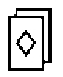
\includegraphics[width=0.05\textwidth]{images/cards.pdf}
	\textit{Die Summe aller Story-Points der beinhalteten Anforderungen}
\end{figure}
\vspace{-15pt}
\begin{figure}[!htb]
		
\includegraphics[width=0.05\textwidth]{images/thumbs.pdf}
	\textit{Die Summe aller Votes der beinhalteten Anforderungen}
\end{figure}
\vspace{-15pt}
\begin{figure}[!htb]
		
\includegraphics[width=0.05\textwidth]{images/files.pdf}
	\textit{Die Anzahl beinhalteten Anforderungen}
\end{figure}

\subsection{Filter/Suche}
Neben diesen Informationen stehen zahlreiche Filter-Methoden und Sortierungs-Methoden zur Verfügung, welche eine Visualisierung über Graphen oder Charts überflüssig machen, da durch diese Methoden alles Nötige ersichtlich ist. Welche Methoden das sind, wird mit Abbildung \ref{fig:header} erklärt.  

\begin{figure}[!htb]
		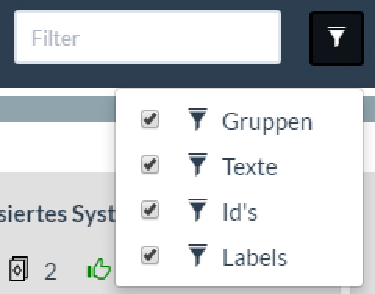
\includegraphics[width=.5\textwidth]{images/filter.pdf}
\centering 
\captionabove[Filter-Methoden]{Filter-Methoden\footnotemark} 
\label{fig:header}
\end{figure}
\footnotetext{Ein Ausschnitt von dem Header des User-Interface mit allen Filter-Methoden}

Hierbei kann eingestellt werden, in welchen Elementen gesucht werden soll.
\begin{description}
\item Gruppen:\\
\textit{Hier wird in allen Gruppennamen gesucht}
\item Texte:\\
\textit{Hier wird in allen Texten, also in den Anforderungsbeschreibungen gesucht}
\item Id's:\\
\textit{Bezieht die Id´s der Anforderungen mit ein}
\item Labels:\\
\textit{Bezieht die Labels mit ein, welche den Anforderungen zugeordnet wurden}
\end{description}

Zudem kann nach mehreren Texten gleichzeitig gesucht werden. Dazu wird für eine \textit{"und"} Verknüpfung ein \textit{", "} und für eine \textit{"oder"} Verknüpfung ein \textit{"; "} verwendet. Hierbei ist zu beachten, dass eine \textit{"und"} Verknüpfung immer höher priorisiert wird. So könnte ein Filter-String wie folgt aussehen:

\begin{quote}
\textit{"Staffelplan, Generierung; Stat, 14"}
\end{quote}

Nach dem deaktivieren des Texte-Filters sieht das Ergebnis wie in Abbildung \ref{fig:filterergebnis} aus.

\begin{figure}[!htb]
		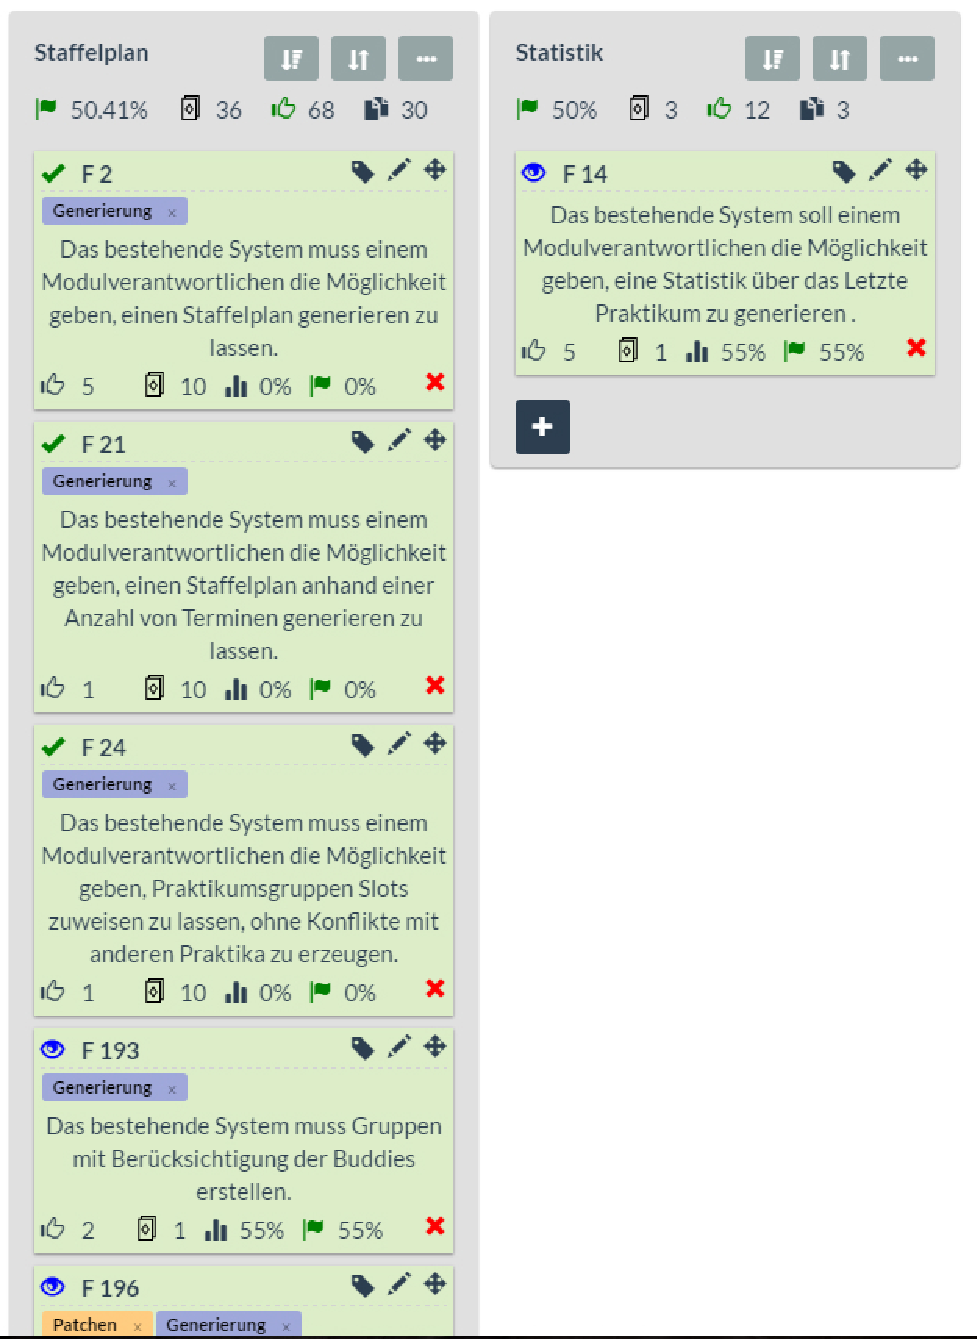
\includegraphics[width=.5\textwidth]{images/filterergebnis.pdf}
\centering 
\captionabove[Filter-Ergebnis]{Filter-Ergebnis\footnotemark} 
\label{fig:filterergebnis}
\end{figure}
\footnotetext{Das Ergebnis der Filterung nach \textit{"Staffelplan, Generierung; Stat, 14"}}

\subsection{Sortierung}
Durch die Kombination der Filter-Methoden mit den Sortierungs-Methoden können beinahe alle möglichen Anfragen erzeugt werden. Auch hier stehen einige Auswahlmöglichkeiten zur Verfügung. Die Abbildungen \ref{fig:sortgruppe}, welche die Sortierung in einer Gruppe anzeigt und \ref{fig:sortgesamt}, auf der die Möglichkeiten für die Sortierung aller Gruppen zu sehen ist, sollten selbsterklärend sein.

\begin{figure}[!htb]
		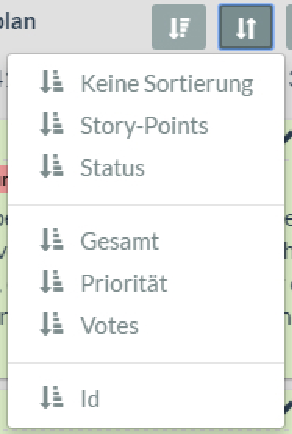
\includegraphics[width=.25\textwidth]{images/sortierunggruppe.pdf}
\centering 
\captionabove[Sortierung innerhalb einer Gruppe]{Sortierung innerhalb einer Gruppe\footnotemark} 
\label{fig:sortgruppe}
\end{figure}
\footnotetext{Ein Ausschnitt des User-Interface, auf dem die Möglichkeiten zur Sortierung innerhalb einer Gruppe zu sehen sind}

\begin{figure}[!htb]
		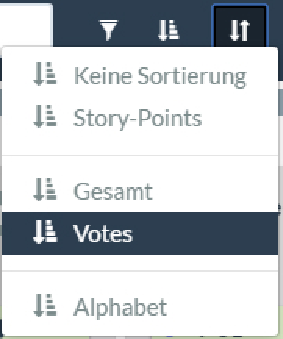
\includegraphics[width=.25\textwidth]{images/sortierunggesamt.pdf}
\centering 
\captionabove[Sortierung gesamt]{Sortierung gesamt\footnotemark} 
\label{fig:sortgesamt}
\end{figure}
\footnotetext{Ein Ausschnitt des User-Interface, auf dem die Möglichkeiten zur Sortierung aller Gruppen zu sehen sind}

\subsection{Sichtbarkeit}
Da sich die Filterung nur auf die Anforderungen selbst bezieht kann es sein, dass nach einer Filterung die Gruppen, welche keine zutreffenden Anforderungen beinhalten, zwar leer sind, jedoch trotzdem angezeigt werden. Dies hat den Grund, dass es durchaus sein kann, dass nach der Filterung eine der gefilterten Anforderungen in eine dann leere Gruppe verschoben werden soll. Ist dies nicht erwünscht besteht die Möglichkeit auch dies zu deaktivieren. Auch die Sichtbarkeit der Anforderungen mit einem bestimmten Status kann eingestellt werden, wie auf Abbildung \ref{fig:sichtbarkeit} zu erkennen ist.

\begin{figure}[!htb]
		
\includegraphics[width=\textwidth]{images/sichtbarkeit.pdf}
\centering 
\captionabove[Sichtbarkeit]{Sichtbarkeit\footnotemark} 
\label{fig:sichtbarkeit}
\end{figure}
\footnotetext{Ein Ausschnitt des User-Interface, auf dem die Möglichkeiten zur Verstellung der Sichtbarkeit zu sehen sind}

All diese Funktionen haben wesentlich zur Bearbeitung und Auswertung der Anforderungen beigetragen und werden es auch noch in Zukunft tun. Diese Web-Anwendung steht unter der Adresse \textit{\href{http://www.req.herborn-software.com}{req.herborn-software.com}} zur Verfügung. Der Login wird nur auf Anfrage vom Verfasser dieses Dokuments vergeben, da Änderungen der Anforderungen direkte Auswirkung auf den Datenbestand haben, und diese Informationen auch nach diesem Projekt weiter verwendet werden.

\nomenclature{Epic}{Die Beschreibung einer Anforderung an eine Software auf einer hohen Abstraktionsebene.\vspace{4mm}}

\chapter{Ergebnisse}

Die Auflistung von 150 Anforderungen wäre an dieser Stelle unangebracht, weshalb hier nur die Top-10 der wichtigsten Anforderungs-Gruppe \textit{"Staffelplan"} aufgeführt werden. Diese Auflistung sollte genug über die Ergebnisse dieser Arbeit aussagen.\\


\begin{minipage}[t]{.5\textwidth}
	\centering
   		\textbf{1. Platz}\\
   		\vspace{16pt}
		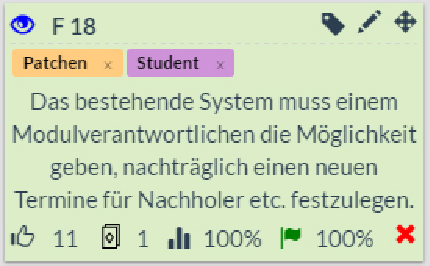
\includegraphics[width=\textwidth]{images/1.pdf}
\end{minipage}
\begin{minipage}[t]{.5\textwidth}
	\centering
   		\textbf{2. Platz}\\
   		\vspace{16pt}
		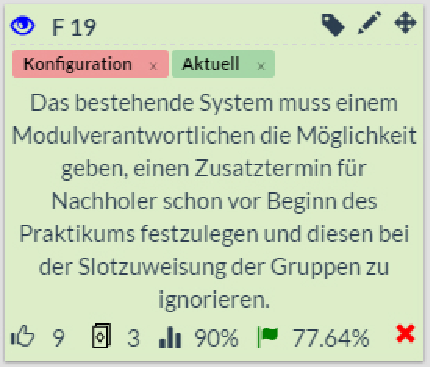
\includegraphics[width=\textwidth]{images/2.pdf}
\end{minipage}



\begin{minipage}[t]{.5\textwidth}
	\centering
   \vspace{16pt}
   		\textbf{3. Platz}\\
   		\vspace{16pt}
		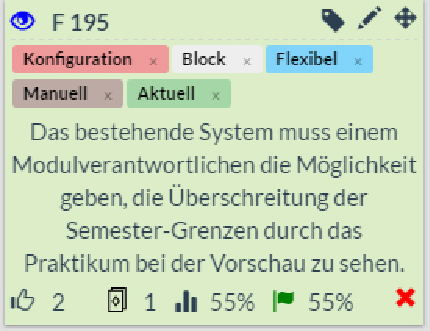
\includegraphics[width=\textwidth]{images/3.pdf}
\end{minipage}
\begin{minipage}[t]{.5\textwidth}
	\centering
   \vspace{16pt}
   		\textbf{4. Platz}\\
   		\vspace{16pt}
		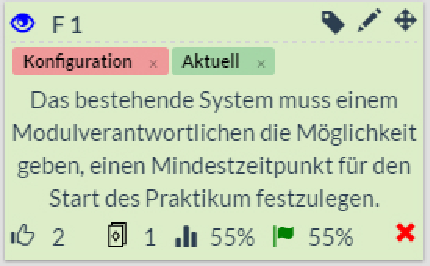
\includegraphics[width=\textwidth]{images/4.pdf}
\end{minipage}



\begin{minipage}[t]{.5\textwidth}
	\centering
   \vspace{16pt}
   		\textbf{5. Platz}\\
   		\vspace{16pt}
		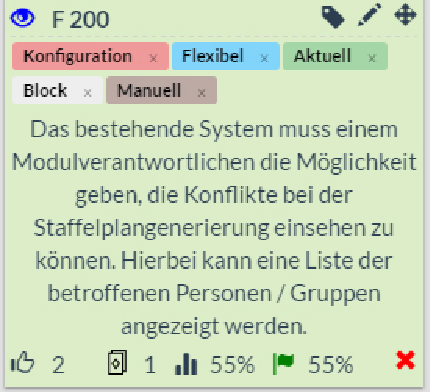
\includegraphics[width=\textwidth]{images/5.pdf}
\end{minipage}
\begin{minipage}[t]{.5\textwidth}
	\centering
   \vspace{16pt}
   		\textbf{6. Platz}\\
   		\vspace{16pt}
		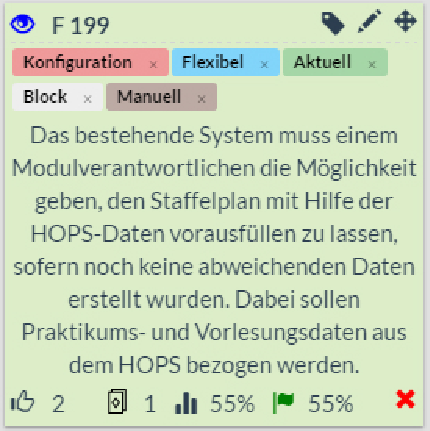
\includegraphics[width=\textwidth]{images/6.pdf}
\end{minipage}



\begin{minipage}[t]{.5\textwidth}
	\centering
   \vspace{16pt}
   		\textbf{7. Platz}\\
   		\vspace{16pt}
		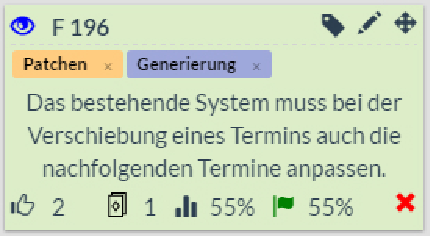
\includegraphics[width=\textwidth]{images/7.pdf}
\end{minipage}
\begin{minipage}[t]{.5\textwidth}
	\centering
   \vspace{16pt}
   		\textbf{8. Platz}\\
   		\vspace{16pt}
		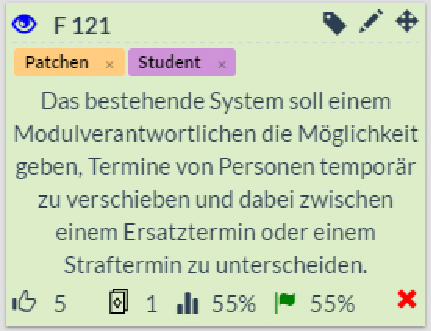
\includegraphics[width=\textwidth]{images/8.pdf}
\end{minipage}



\begin{minipage}[t]{.5\textwidth}
	\centering
   \vspace{16pt}
   		\textbf{9. Platz}\\
   		\vspace{16pt}
		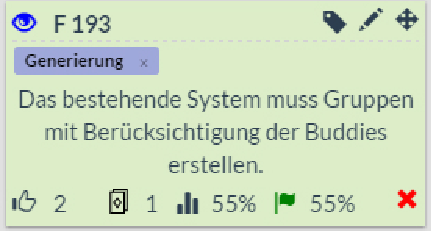
\includegraphics[width=\textwidth]{images/9.pdf}
\end{minipage}
\begin{minipage}[t]{.5\textwidth}
	\centering
   \vspace{16pt}
   		\textbf{10. Platz}\\
   		\vspace{16pt}
		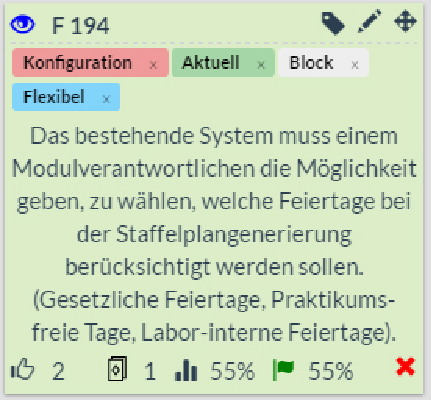
\includegraphics[width=\textwidth]{images/10.pdf}
\end{minipage}

\chapter*{Fazit}
\addcontentsline{toc}{chapter}{Fazit}

Dieses Projekt hatte das Ziel, Anforderungen für das \ac{LWM} zur Verbesserung der Nutzbarkeit und Erweiterung des Nutzerkreises zu ermitteln. Dazu wurden Interviews mit den potentiellen neuen Usern und den bisherigen Nutzern durchgeführt. Die dort entstandenen Ergebnisse wurden zu einer soliden Grundlage für die weitere Entwicklung des Tools aufgearbeitet.\\

Die in dieser Arbeit hervorgebrachten Ergebnisse sollten mit Hilfe weiterer Methoden, wie dem Brainstorming oder anderen, erweitert und verfeinert werden. Zwar sind alle Entwickler des \ac{LWM} selbst Studenten, dennoch reichte das nicht aus, um wirklich alle Anforderungen der Studenten abzudecken. Hierzu hätte man, sofern es Zeitlich möglich gewesen wäre, mit Fragebögen auch die Studenten an dieser Anforderungserhebung teilnehmen lassen können.\\

Diese Arbeit bringt hervor, dass bei vielen Modulen, die dieses Tool noch nicht nutzen ein Interesse zur Nutzung vorhanden ist. Allerdings war dieses den Modulverantwortlichen bislang nicht bekannt, oder die benötigten Funktionen sind in der derzeitigen Anwendung noch nicht implementiert. Durch die Implementierung der hier ermittelten Anforderungen wäre es denkbar, auch diese Module als Nutzer zu gewinnen.\\

Des Weiteren stellte sich heraus, dass das Programm auch bei den aktuellen Nutzern teilweise Wünsche offen lässt, weshalb die Berücksichtigung der hier erlangten Erkenntnisse auch die Zufriedenheit der jetzigen Nutzer steigern könnte. \\

Durch diese Arbeit wird deutlich, dass die Anforderungsanalyse ein wichtiger Schritt in der Software-Entwicklung ist. Durch die sorgfältige Durchführung kann nicht nur die Usability einer Anwendung maßgeblich verbessert werden, sondern auch das Interesse bei einer viel größeren Nutzerzahl geweckt werden. Und gerade letzteres ist meistens der wichtigste Anreiz bei der Entwicklung einer Software.\\
Denn was ist schon eine Software ohne Nutzer?

\singlespacing
%!TEX root = ../draft.tex

  
  	%Erzeugt ein Abbildungsverzeichnis
	\listoffigures
	%Fügt die Zeile "`Abbildungsverzeichnis"' als Chapter ins Inhaltsverzeichnis ein
	\addcontentsline{toc}{chapter}{Abbildungsverzeichnis}
	
	
	%Erzeugt ein Glossar
	\printnomenclature
	%Fügt die Zeile "`Glossar"' als Chapter ins Inhaltsverzeichnis ein
	%\addcontentsline{toc}{chapter}{Glossar}
	
	\chapter*{Abkürzungsverzeichnis}
	\addcontentsline{toc}{chapter}{Abkürzungsverzeichnis}
	\begin{acronym}[FPGA]
	 \setlength{\itemsep}{-\parsep}
	 \acro{LWM}{Labwork Management}
	 \acro{RE}{Requirements Engineering}
	 \acro{MCI}{Mensch-Computer-Interaktion}
	 \acro{US}{User-Story}
	 \acro{SP}{Story-Points}
	 \acro{FPA}{Function-Point-Analyse}
	 \acro{FP}{Function-Points}
	 \acro{SHK}{studentische Hilfskräfte}
	 \acro{WHK}{wissenschaftliche Hilfskräfte}
	\end{acronym}		
		
	%Ändert den Stil des Literaturverzeichnisses
	\bibliographystyle{geralpha}
	%Erzeugt das Literaturverzeichnis anhand der Datei "`literatur.bib"'
	\pagebreak
	\addcontentsline{toc}{chapter}{Literaturverzeichnis}
	\bibliography{literatur}
	%Fügt die Zeile "`Literaturverzeichnis"' als Chapter ins Inhaltsverzeichnis ein
  
  	
\nocite{*}

%=== Schlussteil =====================================================
% \backmatter
% \pagenumbering{Roman}

\setcounter{table}{1}
\setcounter{figure}{1}
%!TEX root = ../draft.tex

\begin{appendices}
% \adjustmtc 
\renewcommand{\appendixname}{ANHANG}
\renewcommand{\appendixtocname}{\appendixname} 
\addappheadtotoc 

% \begin{mtchideinmaintoc}[0]   %  [-1] Den folgenden Inhalt nicht im großen Inhaltsverzeichnis zeigen, [0] ab Chapter im großen Inhaltsverzeichnis anzeigen

\part*{Anhang}

\chapter{Fragebogen}
\label{anh:fragebogen}

\begin{figure}[!htb]
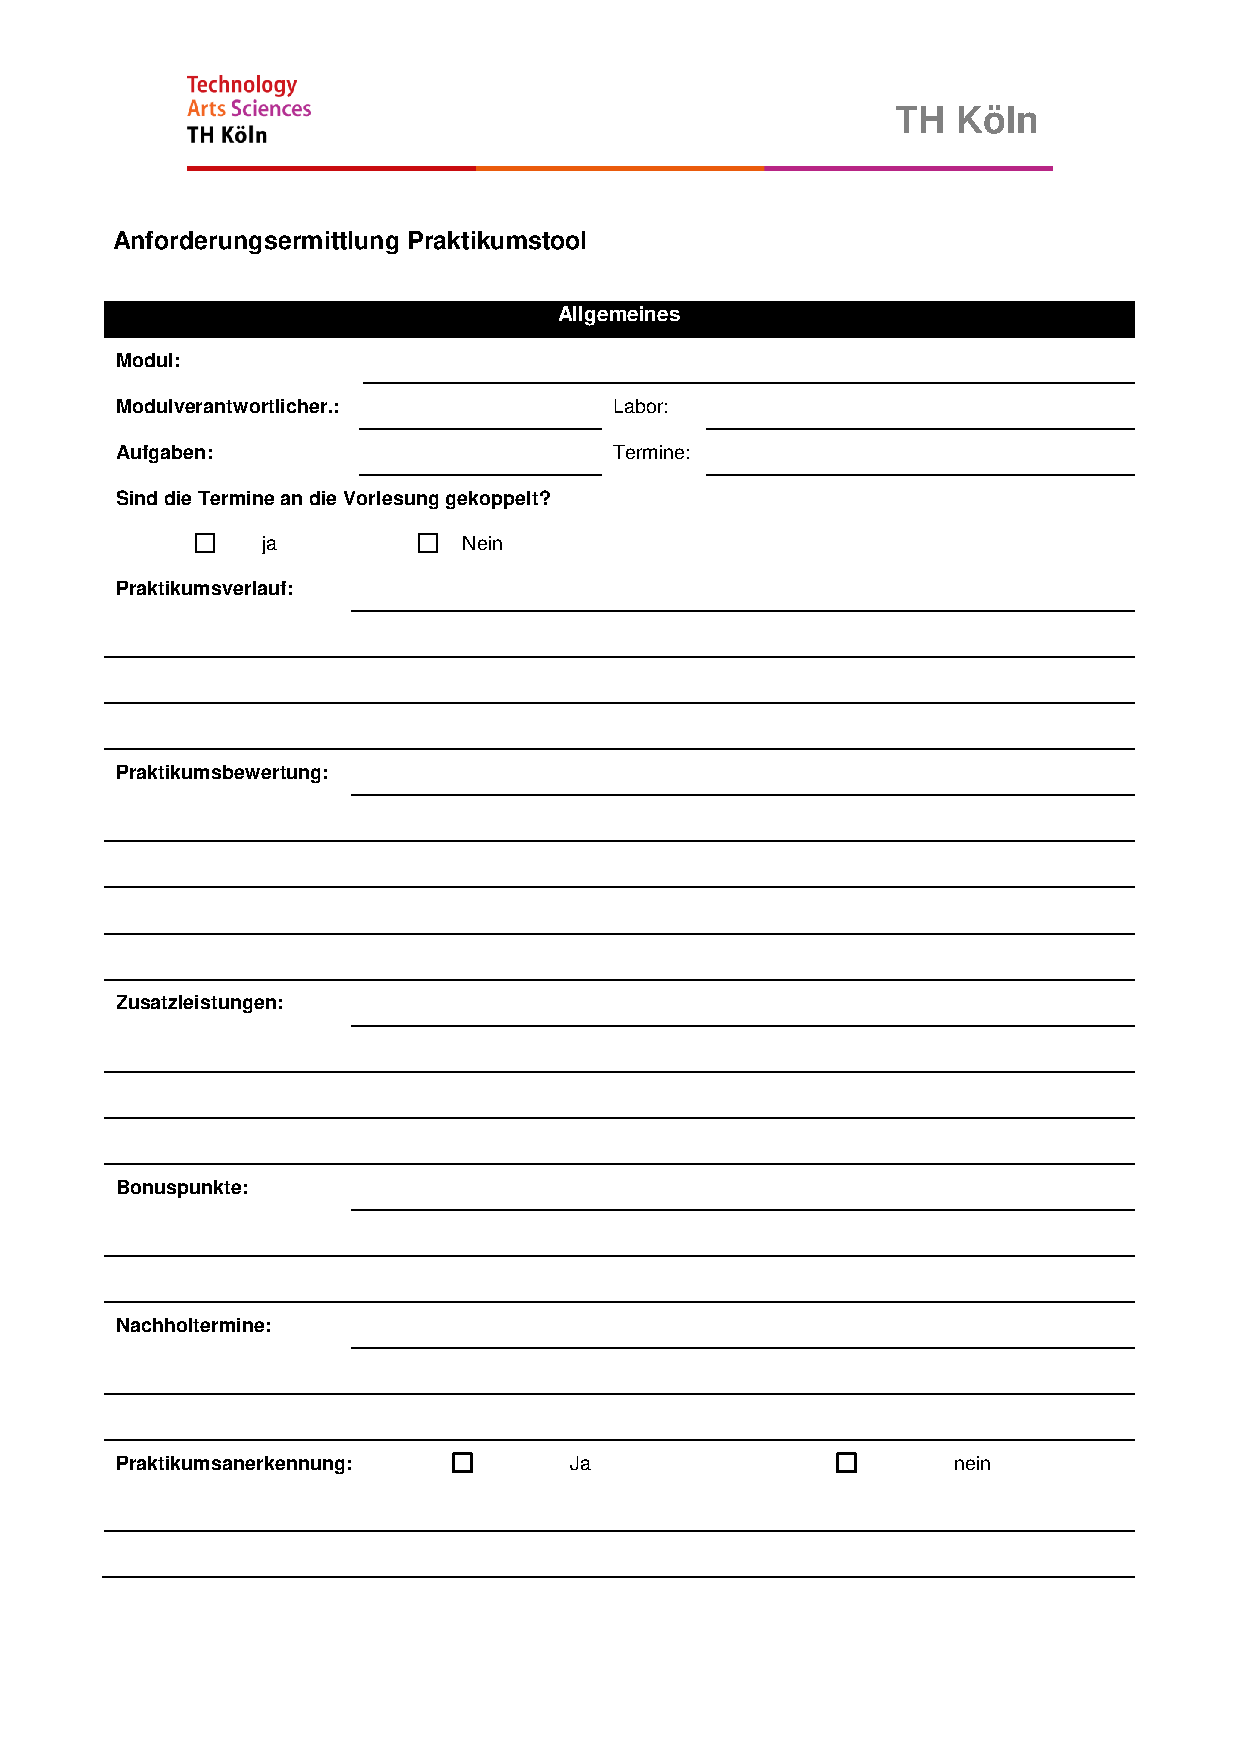
\includepdf[pages=1, width=.95\textwidth]{anhang/Fragebogen.pdf}
\end{figure}

\includepdf[pages=2, width=.95\textwidth]{anhang/Fragebogen.pdf}

\end{appendices}


\setcounter{table}{1}
\setcounter{figure}{1}
%!TEX root = ../draft.tex
\chapter*{Eidesstattliche Erklärung}
\addcontentsline{toc}{chapter}{Eidesstattliche Erklärung}
Ich versichere, die von mir vorgelegte Arbeit selbständig verfasst zu haben.\\ \\
Alle Stellen, die wörtlich oder sinngemäß aus veröffentlichten oder nicht veröffentlichten Arbeiten anderer entnommen sind, habe ich als entnommen kenntlich gemacht. Sämtliche Quellen und Hilfsmittel, die ich für die Arbeit benutzt habe, sind angegeben.\\ \\
Die Arbeit hat mit gleichem Inhalt bzw. in wesentlichen Teilen noch keiner anderen Prüfungsbehörde vorgelegen.
\vspace{1.5cm}
\\
Gummersbach, 14. Juni 2017\\
\begin{figure}[!htb]
		
\includegraphics[width=0.3\textwidth]{images/Unterschrift.pdf}
\end{figure}

Florian Herborn



% chapter eidesstattliche_erklärung (end)

\end{document}